% Submission master (Elsevier, CMAME; journal confirmed 11 Oct 2026).  elsarticle.cls / elsarticle-num.bst (CTAN 2026) are included
% in this folder; Overleaf and TeX Live also provide them.
% Local compile check without elsarticle: check.tex (same sections, article class).
\documentclass[preprint,12pt]{elsarticle}
\usepackage{lmodern}   % 13 Oct (pm): Type-1 Latin Modern fonts with the T1 encoding that elsarticle loads (otherwise bitmap EC fonts on installations without cm-super)
\usepackage{url}
\usepackage{adjustbox,array,tikz,algorithm,algpseudocode}\usetikzlibrary{positioning}
\usepackage{amsmath,amssymb,amsthm,booktabs,graphicx,xcolor,hyperref}\usepackage[expansion=false]{microtype}
\setlength{\emergencystretch}{3em}
\hypersetup{hidelinks}   % 13 Oct (Astra): no coloured link boxes
\newtheorem{lemma}{Lemma}\newtheorem{proposition}{Proposition}\newtheorem{remark}{Remark}
\newcommand{\todo}[1]{\textcolor{red}{[TODO: #1]}}
% 12 Oct: elsarticle's \ref of an appendix section already reads "Appendix X"; the article class (check.tex) gives "X".
\makeatletter\@ifclassloaded{elsarticle}{\newcommand{\appref}[1]{\ref{#1}}}{\newcommand{\appref}[1]{Appendix~\ref{#1}}}\makeatother

% elsarticle appends a period to \paragraph headings; the sources already end them with one, so use the article-class form
\makeatletter\renewcommand\paragraph{\@startsection{paragraph}{4}{\z@}{3.25ex \@plus1ex \@minus.2ex}{-1em}{\normalfont\normalsize\bfseries}}\makeatother
% float placement (Astra, 11 Oct: tables drifted to the end): allow larger top floats and float pages
\renewcommand{\topfraction}{0.85}\renewcommand{\bottomfraction}{0.6}\renewcommand{\textfraction}{0.1}\renewcommand{\floatpagefraction}{0.75}
\setcounter{topnumber}{3}\setcounter{totalnumber}{5}
\journal{Computer Methods in Applied Mechanics and Engineering}
\begin{document}
\begin{frontmatter}
\title{Operator-adapted learned multigrid cycles for high-contrast elliptic problems: accuracy, failure modes and cost}
\author[aff1]{Kumar Kaushik Ranjan\corref{cor1}}
\ead{kumarr@tmi.tolani.edu}
\cortext[cor1]{Corresponding author}
% 13 Oct: affiliation and corresponding e-mail given by the author; postal address to be confirmed by the author.
\affiliation[aff1]{organization={Department of Mechanical Engineering, Tolani Maritime Institute},
            addressline={Induri, Talegaon Dabhade},
            city={Pune},
            postcode={410507},
            state={Maharashtra},
            country={India}}
\begin{abstract}
% Abstract.  v6, 13 Oct 2026 (FINAL_SUBMISSION_REVIEW_ASTRA: no baseline claim; paired-metric qualification on barriers;
% residual-polynomial containment; ~220 words).  Numbers: tables/numbers.txt (tab_core, tab_initseeds, tab_avt, tab_loads, tab_cost).
We study what learned smoothing adds to a multigrid correction for high-contrast elliptic problems on unstructured finite
element meshes. Transfers and Galerkin coarse operators are computed from each sample's operator; only the smoothers are
learned. The architecture represents the classical cycles with fixed, level-independent polynomial smoothers of bounded
degree and combines near-kernel deflation with an energy-norm safeguard relative to a supplied coarse approximation. With four update stages per smoother, one learned pass reduces the energy error relative
to a degree-four Chebyshev-smoothed reference on the same hierarchy by paired geometric-mean factors of about ten on
conductive channels and two on insulating barriers, reproducibly across data seeds and training runs.
The advantage depends strongly on the classical smoothing budget: sixteen-step Chebyshev smoothing narrows it to 1.8 on
channels and reverses the paired advantage on barriers, and three classical passes are more accurate on both at about a
third of the learned pass's time. A network trained with one load loses its advantage on other loads; training on a load
distribution restores a six-fold gain within that distribution. Floating islands retain substantial error. On the tested
CPU configurations the implementation is 12--98 times slower than two-grid or algebraic-multigrid preconditioned conjugate
gradients at matched accuracy. The study separates the contribution of learned smoothing within a prescribed multilevel pass
from practical solver efficiency.

\end{abstract}
\begin{keyword} operator learning \sep multigrid \sep operator-adapted wavelets \sep high contrast \sep deflation \sep finite elements \end{keyword}
\end{frontmatter}
% Section 1 -- introduction.  v3, 13 Oct 2026 (FINAL_SUBMISSION_REVIEW_ASTRA: compressed; three contributions; residual-polynomial
% wording; no baseline-superiority claim).  Numbers: manuscript/tables/numbers.txt.
\section{Introduction}\label{sec:intro}
Many tasks in computational mechanics solve the same elliptic problem for many coefficient fields: uncertainty
quantification for random media, inverse problems and design loops over heterogeneous materials. Neural operators
\cite{kovachki2023,li2021fno,tripura2023wno} promise to amortise such solves by learning the map from coefficient to
solution. At high contrast this is difficult. When the coefficient varies by four orders of magnitude or more, a small nodal
error can hide a large error in the energy norm, the norm in which the discrete problem is posed and in which multigrid and
coarse-space theory measure accuracy. Learned surrogates are moreover often compared with classical methods that receive
less information or are not run to a matched accuracy, which overstates their benefit \cite{mcgreivy2024,chatain2025}.

Classical solvers treat high contrast with operator-dependent multilevel structure. Algebraic multigrid builds its
interpolation from the matrix \cite{vanek1996,xu2017acta}; operator-adapted wavelets
\cite{amaratunga2006,sudarshan2006,sudarshan2005thesis,dheedene2005thesis} and gamblets \cite{owhadi2017} decompose the
solution space into levels that are energy-orthogonal for the given operator; localized orthogonal decomposition and
spectral coarse spaces make the coarse level robust to the contrast
\cite{malqvist2014,peterseim2016,hellman2017,galvis2010,spillane2014geneo}. Learned multigrid methods keep this structure
and learn some of its components, but they iterate the resulting cycle or use it as a preconditioner
\cite{greenfeld2019,luz2020,huang2023,wangluo2026,zhanglisaad2026}. We ask a narrower, architectural question. Given one
pass through a fixed multilevel architecture on a hierarchy adapted to the operator of each sample, can learned smoothers
make that pass measurably more accurate than the same pass with classical smoothers, when both use the same hierarchy,
coarse solution and correction ingredients? How does that answer depend on the classical smoothing budget, and what does the
learned accuracy cost compared with classical solvers run to the same accuracy?

To answer it we construct OA-VCB, a learned V-cycle on an unstructured finite element hierarchy
(Section~\ref{sec:method}). Its transfers are computed from the operator of each sample by a few Jacobi steps towards the
ideal, Schur-complement prolongation of operator-adapted wavelets; its coarse operators are Galerkin products; its coarsest
level is solved exactly. The only learned parts are the smoothers, small nonlinear networks that see the residual and the
local operator weights. Floating conductive regions, whose indicator functions are near-kernel vectors of the operator, are
detected from the matrix and deflated, and the output is the Galerkin projection of the cycle's directions. Every learned
result is paired, sample by sample, with a \emph{classical reference}: the same cycle with degree-four Chebyshev smoothers
and the same coarse solution, deflation and output projection.

Our contributions are the following.
\begin{itemize}
\item A learned V-cycle for unstructured finite element discretisations of high-contrast elliptic problems whose transfers,
coarse operators and deflation vectors are computed from each operator. With $\nu$ update stages per smoother it represents
every classical cycle on the same hierarchy whose smoothers have a fixed, level-independent residual polynomial of degree at
most $\nu$, including weighted Jacobi and fixed-interval Chebyshev smoothing; it is positively homogeneous in the load; and
its output is never worse in the energy norm than the coarse approximation it starts from (Section~\ref{sec:method}).
\item A controlled paired evaluation on three held-out data seeds. With four update stages per pre- and post-smoother, one
learned pass is about ten times more accurate in the energy norm than the degree-four Chebyshev reference on conductive
channels ($G = 9.7$--$10.2$, more accurate on every test sample; $9.7$--$10.7$ over three training initialisations) and about
twice as accurate on insulating barriers (Section~\ref{sec:accuracy}). The margin depends strongly on the classical smoothing
budget: sixteen Chebyshev steps narrow it to $1.8$ on channels and reverse the paired advantage on barriers, and three
classical passes are more accurate than the learned pass on both families at about a third of its time
(Section~\ref{sec:avt}). Ablations show that the
operator-adapted transfers, the near-kernel deflation, the Galerkin output and the nonlinearity of the smoothers each
contribute under this training protocol (Section~\ref{sec:design}).
\item A measured account of the limits (Sections~\ref{sec:cost} and~\ref{sec:failure}): a fixed-load network loses its
advantage on other loads, while distributional training restores it on that distribution; substantial error remains on
floating islands, which a harmonic enrichment with a prespecified written protocol reduces only modestly; and on one CPU the
implementation is one to two orders of magnitude more expensive than converged-to-target classical solvers at matched
accuracy, with no break-even on the tested configurations.
\end{itemize}
Our objective is to isolate the contribution of learned smoothing within an operator-adapted multilevel construction. The
matched classical reference is a control for this architectural question, not a claim of equal work; practical solver
comparisons are made separately, at matched accuracy, and give no computational reason to replace the tested solvers with
OA-VCB. The structural properties are proved; the accuracy results are empirical, and we give no convergence or
approximation theory for the learned smoothers. Learned operator baselines of similar size, adapted to this setting, are
reported for context in \appref{app:baselines}; their rows assess our adaptations, not the published architectures on their
own benchmarks. Section~\ref{sec:related} reviews related work and Section~\ref{sec:discussion} draws the implications of the results
for the design and evaluation of learned multilevel components.

% Section 2 -- related work.  Draft v2, 13 Oct 2026 (positioning table moved to Appendix B).  Every work cited here was checked against its arXiv / publisher page
% on 11 Oct 2026; Table 1 states only what the cited descriptions state (entries to be re-checked against the full texts).
\section{Related work}\label{sec:related}

\paragraph{Neural operators.} Neural operators learn maps between function spaces from samples
\cite{kovachki2023,lu2021deeponet}. Spectral and wavelet variants act on uniform grids: the Fourier neural operator
\cite{li2021fno}, the wavelet neural operator \cite{tripura2023wno} and lifting-based multiresolution operators
\cite{pandey2026lino}; general geometries are handled by deforming the domain onto a latent grid \cite{li2023geofno}, by
message passing on the mesh \cite{pfaff2021}, or by attention over learned groupings of the mesh points
\cite{wu2024transolver}. Multigrid structure has entered operator learning mainly as a parameterisation: MgNet relates
convolutional networks to multigrid \cite{hexu2019mgnet}, and MgNO parameterises the linear operators between neurons by
multigrid cycles with learned convolutional restriction and prolongation \cite{he2024mgno}; hybrid variants correct the
output of a low-order solver with such a network \cite{hu2025hmgno}. In all of these the inter-level transfers, if any, are
learned or fixed by the grid; none of them is computed from the operator of the sample at hand. Experiment-design
critiques \cite{mcgreivy2024,chatain2025,zhang2026breakeven} have shown that comparisons against weak or unmatched classical
baselines overstate the benefit of learned PDE solvers. We therefore compare OA-VCB with a classical reference that uses the same operator-dependent hierarchy and correction
ingredients, and report cost against converged-to-target solvers (Section~\ref{sec:cost}).

\paragraph{Learned multigrid and learned preconditioners.} A second line keeps the iterative solver and learns some of its
components. Learned prolongations for geometric multigrid \cite{greenfeld2019}, learned restriction and prolongation
matrices \cite{katrutsa2017}, learned algebraic-multigrid prolongations predicted by graph networks \cite{luz2020}, and
learned smoothers \cite{huang2023,fanaskov2021} are trained to reduce the error-propagation of a cycle that is then
iterated. Recent work learns smoothing and transfer operators with graph convolutions \cite{wangluo2026}, learns the
smoothing, restriction and interpolation operators of an algebraic-multigrid-type hierarchy for use as a preconditioner
\cite{zhanglisaad2026}, or tunes smoother parameters inside an algebraic multigrid pressure solver with a graph network
\cite{chillon2026}. Other hybrids interleave a neural operator with relaxation sweeps \cite{zhang2024hints}, modify an
iterative solver while preserving its convergence \cite{hsieh2019}, combine a U-Net with a multigrid solver
\cite{han2024ugrid}, or use a neural operator as a preconditioner or coarse correction inside a Krylov method
\cite{rudikov2024,kopanicakova2025,melchers2026,liu2025nodal}. These methods are evaluated as iterative or preconditioned solvers, with convergence and cost assessed at prescribed
tolerances. Our setting is different: one pass through a fixed multilevel architecture, and the accuracy reached by that
pass. We do not learn the transfers; we compute them deterministically from the operator of each sample and learn only the
smoothers. The architecture then represents the classical cycles with fixed polynomial smoothers on the same hierarchy
(Proposition~\ref{prop:containment}), which makes a controlled comparison with classical smoothing possible. Table~\ref{tab:related}
summarises the learned components, transfers and use of the methods cited here.
% Hand-written positioning table (not generated from results).  Entries state only what the cited descriptions state.
\begin{table}[tbp]\centering\footnotesize\setlength{\tabcolsep}{4pt}
\caption{Learned components, inter-level transfers and use of related learned methods, as described in the cited works.
``One pass'': a fixed evaluation returns the approximation; ``iteration'': the learned part is applied inside an iterative
or Krylov solver run to a tolerance; ``precond.'': inside a Krylov method as a preconditioner.}\label{tab:related}
\begin{tabular}{@{}>{\raggedright\arraybackslash}p{0.27\linewidth}>{\raggedright\arraybackslash}p{0.25\linewidth}>{\raggedright\arraybackslash}p{0.25\linewidth}>{\raggedright\arraybackslash}p{0.15\linewidth}@{}}\toprule
method & learned component & inter-level transfers & use \\\midrule
FNO, WNO, LiNO \cite{li2021fno,tripura2023wno,pandey2026lino} & whole map (uniform grid) & none, or a fixed or learned transform & one pass \\
MeshGraphNet-type GNN, Transolver \cite{pfaff2021,wu2024transolver} & whole map (mesh) & none & one pass \\
MgNO \cite{he2024mgno} & multigrid-parameterised linear layers & learned convolutions & one pass \\
Greenfeld et al.\ \cite{greenfeld2019}; Katrutsa et al.\ \cite{katrutsa2017} & prolongation (and restriction) & learned & iteration \\
Luz et al.\ \cite{luz2020} & algebraic-multigrid prolongation & learned (graph network) & iteration \\
Huang et al.\ \cite{huang2023} & smoothers & geometric & iteration \\
UGrid \cite{han2024ugrid} & U-Net iterator built on a multigrid structure & fixed by the grid & iteration \\
Fanaskov \cite{fanaskov2021} & smoothers, and transfers in some variants & fixed or learned & iteration \\
Chill\'on et al.\ \cite{chillon2026} & smoother parameters & algebraic multigrid & iteration \\
Wang and Luo \cite{wangluo2026} & smoothing and transfer operators & learned (graph convolutions) & iteration \\
Zhang, Li and Saad \cite{zhanglisaad2026} & smoothing, restriction, interpolation & learned & precond. \\
HINTS, FCG-NO, DeepONet preconditioners \cite{zhang2024hints,rudikov2024,kopanicakova2025} & neural operator & -- & iteration \\
Melchers et al.\ \cite{melchers2026} & neural coarse correction & fixed coarse basis & precond. \\
\midrule
OA-VCB (this work) & smoothers (nonlinear, operator-informed) & operator-adapted, computed from each $A$ & one pass \\
\bottomrule\end{tabular}
\end{table}


\paragraph{Operator-adapted multiresolution and high-contrast coarse spaces.} The transfers of Section~\ref{sec:routev} come
from operator-adapted finite element wavelets \cite{sudarshan2003,sudarshan2005proc,amaratunga2006,sudarshan2006,sudarshan2005thesis,dheedene2005thesis}
and gamblets
\cite{owhadi2017,owhadi2019book}, whose multilevel decomposition is the exact Schur-complement recursion of
Lemma~\ref{lem:routev}; operator-adapted wavelets have since been extended to finite-element differential forms
\cite{budninskiy2019}, to material-adapted bases and preconditioners for heterogeneous elasticity \cite{chen2019tog,chen2021tog}
and to multiscale electromagnetics \cite{sik2025}. The same objects appear as ideal interpolation in algebraic multigrid \cite{vanek1996,xu2017acta}.
For high-contrast coefficients the localisation of such bases depends on the contrast unless the coarse space resolves the
high-conductivity structures, and contrast-robust coarse spaces add spectral or problem-adapted functions
\cite{malqvist2014,kornhuber2018,peterseim2016,hellman2017,galvis2010,spillane2014geneo,babuska2011,chung2018cem,ma2022}.
Deflation \cite{frank2001,tang2009} targets the low-energy components represented by the selected vectors; the indicator deflation of
Section~\ref{sec:deflation} is the simplest instance, and Section~\ref{sec:islands} measures what it leaves. Neural networks
have been used to approximate these constructions: to map coefficients to compressed operators or to localized orthogonal
decomposition surrogates \cite{kropfl2021,kropfl2022,kropfl2025}, to predict generalised multiscale finite element subspaces
\cite{rudikov2025lsino}, and to learn operators with losses equivalent to errors in problem-adapted norms \cite{qiu2025}.
These works learn the coarse space or the coarse operator; here the operator-adapted hierarchy is computed deterministically from each
sample, using the approximate transfers of \eqref{eq:jacobi}, and the learning acts on the residuals that remain after it.

% Section 3 -- the method.  Draft 5 Oct 2026; 13 Oct: numerical checks and implementation details moved to Appendix A (app:impl).  Every statement here is checked numerically in mathcheck/ (file named
% at the end of each property).  Terminology (review of 5 Oct): the exact route-V transfer is the REFERENCE
% construction; the network uses an inexpensive approximation of it ("route-V-inspired"), never "a gamblet construction".
\section{An operator-adapted learned V-cycle}\label{sec:method}

\subsection{Setting}\label{sec:setting}
We consider the family of elliptic problems
\begin{equation}\label{eq:pde}
  -\nabla\cdot\big(K(x)\nabla u\big) = f \quad\text{in } \Omega, \qquad u = 0 \text{ on } \Gamma_D,
  \qquad K\nabla u\cdot n = 0 \text{ on } \Gamma_N,
\end{equation}
with a symmetric, uniformly positive definite coefficient $K$ that is piecewise constant on the elements and may vary
by several orders of magnitude (isotropic $K = a\,I$ with high-contrast channels or barriers, or tensor-valued, strongly
anisotropic tows); a preliminary plane-strain elasticity case is treated in the same way (\appref{app:settings}). Starting from an
unstructured coarse triangulation $\mathcal{T}_0$ of $\Omega$, $L$ uniform refinements give nested $P_1$ spaces
$V_0\subset V_1\subset\cdots\subset V_L$. On level $k$ the nodes of $V_{k-1}$ (``coarse'', $C$) are ordered before the
nodes created by the refinement (``fine'', $F$), and the geometric prolongation is
$P_k = \begin{bmatrix} I \\ P_{k,F}\end{bmatrix}$, $P_{k,F}$ being nodal interpolation at edge midpoints.

On the finest level the discrete problem is $A u = F$, $A = A_L$ symmetric positive definite. A Galerkin solve on the
level-$k_0$ space gives $u_c$; we write $r = F - A u_c$ and $e = u - u_c = A^{-1} r$. The learned map studied here
returns a correction $c = \mathcal{N}(r; A)\approx e$ in one pass. The case $k_0 = 0$ means that \emph{no external coarse
solution is supplied} ($u_c = 0$, $r = F$); the network still contains its own exact coarsest-level solve.

Table~\ref{tab:notation} collects the notation.
\begin{table}[tbp]\centering\footnotesize
\caption{Notation.}\label{tab:notation}
\begin{tabular}{@{}>{\raggedright\arraybackslash}p{0.27\linewidth}>{\raggedright\arraybackslash}p{0.68\linewidth}@{}}\toprule
$A = A_L$, $A_k$ & fine operator; Galerkin operator on level $k$ ($A_0$ coarsest, solved exactly) \\
$D_k$, $W_{ij}$ & diagonal of $A_k$; normalised couplings $A_{ij}/A_{ii}$ (smoother inputs) \\
$P_k$, $\widehat\Phi_k$, $\Phi_k^\star$ & geometric, computational (eq.~\eqref{eq:jacobi}) and ideal (eq.~\eqref{eq:ideal}) prolongation \\
$u$, $u_c$, $r$, $e$ & discrete solution, level-$k_0$ Galerkin approximation, $r = F - Au_c$, $e = u - u_c$ \\
$Z$, $x_0$ & near-kernel indicator vectors; deflation \eqref{eq:deflation} \\
$x, x_c, x_p$ & pre-smoothing, coarse-correction and post-smoothing parts of the finest-level cycle \\
$\mathcal{S}^{\mathrm{pre}}, \mathcal{S}^{\mathrm{post}}$ & learned smoothers \eqref{eq:smoother} \\
$\|v\|_A$, $e(\hat u)$ & energy norm $\sqrt{v^\top Av}$; relative energy error $\|u - \hat u\|_A/\|u\|_A$ \\
$G$, $W$ (Section~\ref{sec:protocol}) & paired geometric-mean error ratio; win fraction \\
\bottomrule\end{tabular}
\end{table}

\subsection{Reference construction: ideal (route-V) transfers}\label{sec:routev}
Write the level-$k$ operator in the $C/F$ ordering as
$A_k = \begin{bmatrix} A_{CC} & A_{CF}\\ A_{FC} & A_{FF}\end{bmatrix}$ and define
\begin{multline}\label{eq:ideal}
  \Phi_k^\star = \begin{bmatrix} I\\ -A_{FF}^{-1}A_{FC}\end{bmatrix}, \qquad
  E_F = \begin{bmatrix} 0\\ I\end{bmatrix}, \qquad S_k = (\Phi_k^\star)^{\!\top} A_k \Phi_k^\star\\
  = A_{CC}-A_{CF}A_{FF}^{-1}A_{FC}.
\end{multline}
\begin{lemma}[two-level block diagonalisation]\label{lem:routev}
$E_F^\top A_k \Phi_k^\star = 0$, hence
\[
[\Phi_k^\star\;E_F]^\top A_k [\Phi_k^\star\;E_F] = \operatorname{diag}(S_k, A_{FF})
\]
and
\begin{equation}\label{eq:inverse}
  A_k^{-1} = \Phi_k^\star S_k^{-1} (\Phi_k^\star)^{\!\top} + E_F A_{FF}^{-1} E_F^\top .
\end{equation}
\end{lemma}
\begin{proof}
$E_F^\top A_k\Phi_k^\star = A_{FC} - A_{FF}A_{FF}^{-1}A_{FC} = 0$. The matrix $T = [\Phi_k^\star\;E_F]$ is unit block
lower triangular, hence invertible, and $T^\top A_k T$ is block diagonal; inverting
$A_k = T^{-\top}\operatorname{diag}(S_k,A_{FF})T^{-1}$ gives \eqref{eq:inverse}.
\end{proof}
Applied recursively with $A_{k-1} = S_k$, \eqref{eq:inverse} is the exact multilevel decomposition behind
operator-adapted wavelets \cite{amaratunga2006,sudarshan2005thesis,dheedene2005thesis} and, with nodal measurement functions, gamblets
\cite{owhadi2017}: the columns of $\Phi_k^\star$ are $A$-harmonic extensions of the coarse nodal values. It is also the
ideal interpolation of algebraic multigrid. Two remarks fix how it is used here. First, \eqref{eq:inverse} restricts with $\Phi^\top$ and prolongs with $\Phi$, so we
pass residuals down with $\widehat\Phi_k^{\!\top}$ (the contrast with exactly invertible lifting networks is discussed in
\appref{app:impl}). Second, $\Phi_k^\star$ is dense in general and its decay with distance depends on the contrast
unless the coarse space resolves the high-conductivity structures \cite{hellman2017,peterseim2016}. We therefore use
\eqref{eq:ideal} as the reference and compute an inexpensive approximation.

\paragraph{Computational transfer.} Starting from the geometric predict, $m$ weighted-Jacobi steps are applied to
$A_{FF}X = -A_{FC}$:
\begin{equation}\label{eq:jacobi}
  X^{(0)} = P_{k,F}, \quad X^{(j+1)} = X^{(j)} + \omega D_{FF}^{-1}\big(-A_{FC} - A_{FF}X^{(j)}\big), \quad
  \widehat\Phi_k = \begin{bmatrix} I\\ X^{(m)}\end{bmatrix},
\end{equation}
with $D_{FF} = \operatorname{diag}(A_{FF})$, $\omega = 2/3$, $m = 4$ (prolongator smoothing in the sense of smoothed
aggregation \cite{vanek1996}). The number of steps $m$ controls the stencil width of $\widehat\Phi_k$ and how closely it
approximates $\Phi_k^\star$; increasing $m$ approaches the ideal prolongation only when the Jacobi iteration for $A_{FF}$
converges, which symmetric positive definiteness alone does not guarantee for a fixed weight. $m = 4$ was fixed during
development, and its measured effect on the classical reference, the learned margin, the operator complexity and the set-up
time is reported in \appref{app:sensitivity}. The coarse operators are Galerkin, $A_{k-1} = \widehat\Phi_k^{\!\top} A_k\widehat\Phi_k$,
and the hierarchy is computed per sample from $A$ alone.
\begin{proposition}[local reproduction of the kernel]\label{prop:constants}
Let $t$ be a level-$k$ vector with restriction $t_C$ to the coarse nodes (constants for diffusion; translations and
rotations for elasticity, which $P_1$ interpolation reproduces), and let $\mathcal{N}_r(f)$ denote the nodes within $r$
graph steps of a fine node $f$. If $P_k t_C = t$ on $\mathcal{N}_m(f)$ and $(A_k t)_g = 0$ for every fine node
$g\in\mathcal{N}_{m-1}(f)$, then $(\widehat\Phi_k t_C)_f = t_f$.
\end{proposition}
\begin{proof}
Write $\widehat\Phi^{(j)} = [I;X^{(j)}]$; the update in \eqref{eq:jacobi} applied to $t_C$ at a fine node $g$ is
$-\omega\,(A_k\widehat\Phi^{(j)}t_C)_g/A_{gg}$, which depends on $\widehat\Phi^{(j)}t_C$ on $\mathcal{N}_1(g)$ only. We
show by induction that $\widehat\Phi^{(j)}t_C = t$ on $\mathcal{N}_{m-j}(f)$. For $j = 0$ this is the hypothesis. If it
holds for $j$ and $g\in\mathcal{N}_{m-j-1}(f)$, then $\mathcal{N}_1(g)\subset\mathcal{N}_{m-j}(f)$, so the update at $g$ is
$-\omega(A_kt)_g/A_{gg} = 0$ and $\widehat\Phi^{(j+1)}t_C = t$ on $\mathcal{N}_{m-j-1}(f)$. Take $j = m$.
\end{proof}
The statement is graph-local and conditional; the measured reproduction defects of the elasticity transfers, at round-off
on most finest-level rows and growing on coarser levels, are reported in \appref{app:impl}.

\subsection{The learned cycle}\label{sec:cycle}
For $k = L, L-1, \dots, 1$ and a right-hand side $b$ on level $k$, one cycle returns three parts,
\begin{equation}\label{eq:cycle}
\begin{aligned}
  x &= \mathcal{S}^{\mathrm{pre}}(b; A_k), &
  e_c &= \mathcal{C}_{k-1}\big(\widehat\Phi_k^{\!\top}(b - A_k x)\big), &
  x_c &= \widehat\Phi_k e_c, \\
  x_p &= \mathcal{S}^{\mathrm{post}}\big(b - A_k(x + x_c); A_k\big), &
  \mathcal{C}_k(b) &= x + x_c + x_p, & \mathcal{C}_0 &= A_0^{-1},
\end{aligned}
\end{equation}
with an exact dense solve on the coarsest level (28 nodes for the perforated square, 45 for the polygon). Only the smoothers are learned. The transfers are computed deterministically from each sample with the approximate
construction \eqref{eq:jacobi}; the Galerkin operators, residual updates and the coarsest solve are fixed algebraic
operations on them.

\paragraph{Smoother.} A smoother maps a right-hand side $b$ on a level with operator $A_k$ to a correction. With
$d = \operatorname{diag}(A_k)$, $z = b/d$ and $\sigma = \|z\|_{\mathrm{rms}}$, node features are
$(z_i/\sigma,\ \log(d_i/\operatorname{median} d))$; an encoder lifts them to a latent $s\in\mathbb{R}^{n\times C}$, and
$T$ steps of
\begin{equation}\label{eq:smoother}
\begin{aligned}
  s_i \leftarrow s_i &+ \mathcal{L}_t\big([\,s_i,\ \textstyle\sum_{j\ne i} W_{ij} V_t s_j\,]\big)\\
       &+ \mathcal{M}_t\big([\,s_i,\ \textstyle\sum_{j\ne i} W_{ij} V_t s_j,\ \overline{m}_i\,]\big),
  \qquad W_{ij} = A_{ij}/A_{ii},
\end{aligned}
\end{equation}
follow, where $\mathcal{L}_t$ and $V_t$ are linear, $\mathcal{M}_t$ is a small MLP and $\overline{m}_i$ the mean of edge
messages $\mathrm{MLP}([s_i,s_j,\delta_{ij},|\delta_{ij}|,W_{ij}])$ over the neighbours of $i$, with
$\delta_{ij} = (\mathbf{x}_j-\mathbf{x}_i)/h_k$ the edge vector in units of the level's mesh width. The output is $\sigma\cdot\mathrm{dec}(s)$. The operator
enters only through $W$ and $d$ of the level the smoother acts on; one pre- and one post-smoother are shared by all
levels ($T = \nu = 4$, $C$ chosen to meet the parameter budget).

\subsection{Near-kernel deflation from the operator}\label{sec:deflation}
High-contrast media can contain \emph{floating islands}: conductive regions enclosed by low-conductivity barriers and
not connected to $\Gamma_D$. Their indicator vectors $z$ satisfy $z^\top A z/z^\top D z \ll 1$, i.e.\ they lie close to the
kernel of $A$, and the nodal hierarchy used here does not contain them unless its coarse levels resolve the island. We detect
them from $A$ alone. Let $G$ be the graph of strong connections, $-A_{ij}\ge\theta\sqrt{A_{ii}A_{jj}}$ ($\theta = 0.1$). A
connected component of $G$ is \emph{anchored} if one of its rows is strongly coupled to the Dirichlet boundary,
$\sum_j A_{ij}\ge\theta A_{ii}$ (interior rows of a diffusion matrix sum to zero). The indicator of every unanchored
component with Rayleigh quotient $z^\top Az/z^\top Dz<\tau$ ($\tau = 0.05$) is a column of $Z$. Before the cycle,
\begin{equation}\label{eq:deflation}
  x_0 = Z(Z^\top A Z)^{-1}Z^\top r .
\end{equation}
If no vector is detected, $Z$ is empty and $x_0 = 0$ (no deflation); for the elasticity case $Z$ is always empty. The
indicators of distinct components have disjoint supports and positive energy, so $Z^\top AZ$ is nonsingular whenever $Z$ is
not empty.
Against the geometric ground truth (conductive elements, connected components without a Dirichlet node) the detector
has recall 74/75 and precision 75/78 on the barrier test set of the development data seed; the three additional vectors are near-kernel modes by
definition (Rayleigh quotients 0.008--0.015) but not coefficient islands (\texttt{mathcheck/check\_oa\_vcp.log}).
The detector is a heuristic for scalar diffusion matrices: the strength criterion uses negative off-diagonal couplings
and the anchoring test the zero row sums of interior rows. A small Rayleigh quotient certifies that a returned vector has
low energy; it does not certify that every important low-energy direction was found. For tensor coefficients (whose
$P_1$ matrices need not be M-matrices) we report how many vectors it returns, and for elasticity it is not used. The
thresholds were fixed on the development seed and are kept in all main experiments; a subsequent sensitivity check on the
held-out barrier sets (\appref{app:sensitivity}) shows that $\theta$ matters more than $\tau$ and that the learned margin
changes little ($G = 2.03$ against $2.00$ with $\theta = 0.05$).

\subsection{Galerkin output and training}\label{sec:output}
The cycle is applied to the deflated residual $b = r - Ax_0$ on the finest level, and its parts are combined
energy-optimally together with the near-kernel vectors:
\begin{equation}\label{eq:projection}
  W = [\,x,\ x_c,\ x_p,\ Z\,], \qquad c = x_0 + W y, \qquad W^\top A W\, y = W^\top (r - A x_0).
\end{equation}
If the columns of $W$ are linearly dependent (a vanishing part, say), the normal equations remain consistent and
determine $Wy$, the $A$-orthogonal projection onto $\operatorname{span}W$, uniquely, although $y$ need not be unique; as a
mathematical convention we take $y = (W^\top AW)^{+}W^\top(r - Ax_0)$, and any rank-revealing solve gives the same $c$. The small
Gram system and its right-hand side are formed and solved in double precision, after Jacobi scaling of its columns; the
regularisation and acceptance step of the implementation are described in \appref{app:impl}. Training minimises
$\ell(c) + \ell(x_0 + x + x_c + x_p)$ with $\ell$ the mean of the relative $L^2$ and energy errors. The second term keeps
each part of the cycle well scaled; training through the projection alone makes the loss insensitive to the scale of the
parts and stalls on the channel problems (variant \texttt{oa-vcp}, development-stage CPU screen on a two-level mesh, \path{diagnostics_cost/oa_vcp_L2_cpu.log}).

\paragraph{Summary of one pass.} Algorithm~\ref{alg:opdata} lists the operator data computed for each sample and
Algorithm~\ref{alg:pass} one pass of the network; Figure~\ref{fig:schematic} shows how they fit together. Everything except
the two smoothers is a prescribed algebraic operation: the transfers, Galerkin levels, coarsest factorisation and deflation
vectors are computed from the operator of the sample before the pass, while the deflation step, residual updates and output
projection act on the residual and on the parts produced by the smoothers. Both algorithms and the figure show the ideal
mathematical construction, with exact solves of the small deflation and normal-equation systems; the regularisation and
acceptance step of the implementation are described in \appref{app:impl}.
\begin{algorithm}[tbp]
\caption{Operator data for one sample (computed from $A = A_L$; no learned parameters).}\label{alg:opdata}
\begin{algorithmic}[1]
\Require fine operator $A_L$; geometric prolongations $P_k = [I;\,P_{k,F}]$; number of levels; $m = 4$, $\omega = 2/3$
\For{$k = L, L-1, \dots, 1$}
  \State split $A_k$ into $C/F$ blocks; $X \gets P_{k,F}$
  \For{$j = 1,\dots,m$} \State $X \gets X + \omega D_{FF}^{-1}(-A_{FC} - A_{FF}X)$ \Comment{eq.~\eqref{eq:jacobi}} \EndFor
  \State $\widehat\Phi_k \gets [I;\,X]$, \quad $A_{k-1} \gets \widehat\Phi_k^{\!\top}A_k\widehat\Phi_k$ \Comment{Galerkin level}
  \State $d_k \gets \operatorname{diag}(A_k)$, \quad $W^{(k)}_{ij} \gets A_{ij}/A_{ii}$ \Comment{smoother inputs}
\EndFor
\State factor $A_0$ (dense, exact)
\State $Z \gets$ indicators of the unanchored strong-connection components of $A_L$ with Rayleigh quotient $<\tau$ \Comment{Section~\ref{sec:deflation}}
\end{algorithmic}
\end{algorithm}
\begin{algorithm}[tbp]
\caption{One OA-VCB pass, ideal construction (exact small solves; for the regularised implementation see
\appref{app:impl}). $\mathcal{S}^{\mathrm{pre}},\mathcal{S}^{\mathrm{post}}$ are the learned smoothers
\eqref{eq:smoother}, shared by all levels. If $Z$ is empty, $x_0 = 0$; if $W$ is rank-deficient, $y$ is the
pseudoinverse solution, and $Wy$ is unique.}\label{alg:pass}
\begin{algorithmic}[1]
\Require residual $r = F - Au_c$; operator data of Algorithm~\ref{alg:opdata}
\State $x_0 \gets Z(Z^{\!\top}AZ)^{-1}Z^{\!\top}r$, \quad $b \gets r - Ax_0$ \Comment{deflation \eqref{eq:deflation}}
\State $(x, x_c, x_p) \gets \textsc{Cycle}(L, b)$ \Comment{parts on the finest level}
\State $W \gets [\,x,\ x_c,\ x_p,\ Z\,]$; solve $W^{\!\top}AW\,y = W^{\!\top}b$ \Comment{Galerkin output \eqref{eq:projection}}
\State \Return $\hat u = u_c + x_0 + Wy$
\Function{Cycle}{$k$, $b$}
  \If{$k = 0$} \Return $A_0^{-1}b$ \EndIf
  \State $x \gets \mathcal{S}^{\mathrm{pre}}(b; A_k)$
  \State $x_c \gets \widehat\Phi_k\,\textsc{Cycle}\big(k-1,\ \widehat\Phi_k^{\!\top}(b - A_kx)\big)$
  \State $x_p \gets \mathcal{S}^{\mathrm{post}}\big(b - A_k(x + x_c); A_k\big)$
  \State \Return $(x, x_c, x_p)$ if $k = L$, else $x + x_c + x_p$
\EndFunction
\end{algorithmic}
\end{algorithm}
\begin{figure}[tbp]\centering
\resizebox{\linewidth}{!}{% Schematic of OA-VCB (TikZ), 11 Oct 2026.  Input with \input{figures/fig_schematic} inside a figure environment.
\begin{tikzpicture}[x=1cm, y=1cm, font=\footnotesize, >=latex,
  box/.style={draw=black!70, rounded corners=2pt, align=center, inner sep=3pt},
  op/.style={box, fill=black!5},
  learn/.style={box, fill=blue!12, draw=blue!60!black, minimum width=9mm, minimum height=5.5mm},
  lvl/.style={font=\scriptsize, text=black!55}]
% left: operator data
\node[box] (in) at (1.80,2.55) {$r = F - A\,u_c$};
\node[op, text width=40mm] (data) at (1.80,0.15) {\textbf{operator data}, from $A$\\[2pt]
  $\widehat\Phi_k$: $m$ Jacobi steps\\ towards $[I;\,-A_{FF}^{-1}A_{FC}]$\\[2pt]
  $A_{k-1}=\widehat\Phi_k^{\!\top}A_k\widehat\Phi_k$, \ $A_0^{-1}$\\[2pt]
  $Z$: near-kernel indicators\\[2pt] $D_k$, \ $W_{ij}=A_{ij}/A_{ii}$};
% middle: deflation and V-cycle
\node[op] (defl) at (7.70,2.55) {deflation: $x_0 = Z(Z^{\!\top}AZ)^{-1}Z^{\!\top}r$, \ $b = r - Ax_0$};
\node[learn] (s3) at (6.10,1.35) {$\mathcal{S}^{\mathrm{pre}}$};   \node[learn] (p3) at (9.30,1.35) {$\mathcal{S}^{\mathrm{post}}$};
\node[learn] (s2) at (6.65,0.45) {$\mathcal{S}^{\mathrm{pre}}$};  \node[learn] (p2) at (8.75,0.45) {$\mathcal{S}^{\mathrm{post}}$};
\node (s1) at (7.20,-0.35) {$\vdots$};                            \node (p1) at (8.20,-0.35) {$\vdots$};
\node[op, minimum width=9mm] (c0) at (7.70,-1.15) {$A_0^{-1}$};
\draw[->] (s3) -- node[left, lvl] {$\widehat\Phi_L^{\!\top}$} (s2);  \draw[->] (s2) -- (s1);  \draw[->] (s1) -- (c0);
\draw[->] (c0) -- (p1); \draw[->] (p1) -- (p2); \draw[->] (p2) -- node[right, lvl] {$\widehat\Phi_L$} (p3);
\node[lvl, anchor=east] at (5.50,1.35) {level $L$}; \node[lvl, anchor=east] at (5.50,0.45) {level $L{-}1$};
\node[lvl, anchor=east] at (5.50,-1.15) {level $0$};
\draw[->] (defl.south -| s3) -- (s3);
\node[lvl, align=center] at (7.70,-1.85) {learned smoothers, shared by all levels:\\ $\mathcal{S}(b;A_k) = \sigma\,\mathrm{dec}(s)$, eq.~\eqref{eq:smoother}};
% right: Galerkin output
\node[op, text width=40mm] (out) at (13.00,0.30) {\textbf{Galerkin output}\\[2pt]
  $W=[\,x,\ x_c,\ x_p,\ Z\,]$\\[1pt] $W^{\!\top}AW\,y = W^{\!\top}b$\\[1pt] $c = x_0 + Wy$\\[3pt]
  $\|e-c\|_A\le\|e-x_0\|_A\le\|e\|_A$};
\node[box] (res) at (13.00,2.55) {$\hat u = u_c + c$};
% connections
\draw[->] (in) -- (defl);
\draw[->, dashed, black!55] (data.east |- 0,-0.55) -- node[above, lvl] {operators $A_k$, $\widehat\Phi_k$, $Z$} (6.9,-0.55);
\draw[->] (p3.east) -- node[above, lvl] {$x,\ x_c,\ x_p$} (out.west |- p3.east);
\draw[->] (out) -- (res);
\end{tikzpicture}
}
\caption{One OA-VCB pass, ideal construction. Grey boxes denote prescribed algebraic operations; blue boxes denote the learned
smoothers, one pre- and one post-smoother shared by all levels. The operator-data box is precomputed from each sample's
operator (Algorithm~\ref{alg:opdata}); deflation and the Galerkin output depend on the residual and on the cycle's parts. The
output is the energy-optimal combination of the three parts and the near-kernel vectors, which gives the safeguard of
Proposition~\ref{prop:safeguard}; the regularisation and acceptance step of the implementation are described in
\appref{app:impl}.}
\label{fig:schematic}
\end{figure}

\subsection{Properties}\label{sec:properties}
\begin{proposition}[containment of fixed polynomial smoothers]\label{prop:containment}
Let $\nu\ge1$ steps and $C\ge2$ latent channels be given, and let $p(\mu) = \sum_{j=0}^{\nu-1}a_j\mu^j$ be any real
polynomial of degree at most $\nu-1$. Set the encoder, the step maps and the decoder of both smoothers as follows: channel $1$
of the latent carries $z/\sigma$, channel $0$ starts at zero, $V_t$ selects channel $0$, $\mathcal{L}_t$ maps $(s,\,q)$ to
$a_{\nu-t}\,s_1 + q_0$ in channel $0$ and to zero elsewhere, $\mathcal{M}_t = 0$, and the decoder reads channel $0$. Then on
every level each smoother returns
\begin{equation}\label{eq:polysmoother}
\begin{aligned}
  x &= p(B_k)\,D_k^{-1}b, & B_k &= D_k^{-1}A_k,\\
  A_k^{-1}b - x &= R(B_k)\,A_k^{-1}b, & R(\mu) &= 1 - \mu\,p(\mu),
\end{aligned}
\end{equation}
with the same coefficients on all levels; and the network output \eqref{eq:deflation}--\eqref{eq:projection} equals the
classical deflated V$(\nu,\nu)$ cycle with these smoothers, transfers \eqref{eq:jacobi}, Galerkin levels, exact coarsest solve
and Galerkin projection onto $\operatorname{span}\{x,x_c,x_p,Z\}$. Equivalently, every real residual polynomial $R$ of degree at
most $\nu$ with $R(0) = 1$ is represented. When $R$ has real roots $1/\omega_t$, the step maps
$\mathcal{L}_t(s,q) = \omega_t(s_1 - s_0 - q_0)$ in channel $0$ realise the same smoother as the Richardson steps
\begin{equation}\label{eq:richardson}
  x \leftarrow x + \omega_t D_k^{-1}(b - A_k x), \qquad t = 1,\dots,\nu, \qquad x = 0 \text{ initially},
\end{equation}
for which $R(\mu) = \prod_{t=1}^{\nu}(1 - \omega_t\mu)$. Special cases are
\begin{enumerate}
\item[(a)] weighted Jacobi smoothing, $\omega_t = \omega$;
\item[(b)] degree-$\nu$ Chebyshev smoothing on a fixed interval $[\lambda/q,\lambda]$ with $\lambda>0$ and $q>1$,
$\omega_t^{-1} = \theta - \delta\cos\big((2t-1)\pi/(2\nu)\big)$, $\theta = (\lambda + \lambda/q)/2$, $\delta = (\lambda - \lambda/q)/2$,
for which $\prod_t(1-\omega_t\mu) = T_\nu\big((\theta-\mu)/\delta\big)/T_\nu(\theta/\delta)$, the residual polynomial of the
Chebyshev semi-iteration \cite{saad2003}.
\end{enumerate}
\end{proposition}
\begin{proof}
Write $s_0 = x/\sigma$ for channel $0$ at node $i$; its aggregate is $q_0 = \sum_{j\ne i}W_{ij}x_j/\sigma = \big((B_k - I)x\big)_i/\sigma$.
Since the step map is added to the current state, step $t$ of the first construction gives
$s_0 + a_{\nu-t}s_1 + q_0 = \big(B_kx + a_{\nu-t}D_k^{-1}b\big)_i/\sigma$, that is, $x_t = B_kx_{t-1} + a_{\nu-t}D_k^{-1}b$ with
$x_0 = 0$, and Horner's rule gives $x_\nu = \sum_{j=0}^{\nu-1}a_jB_k^{\,j}D_k^{-1}b = p(B_k)D_k^{-1}b$. Multiplying the decoded
channel by $\sigma$ undoes the scaling, and $A_k^{-1}b - p(B_k)B_kA_k^{-1}b = R(B_k)A_k^{-1}b$. Conversely, a real $R$ of degree
at most $\nu$ with $R(0) = 1$ has the form $1-\mu p(\mu)$ with $p$ real of degree at most $\nu-1$. In the second construction
step $t$ gives $s_0 + \omega_t(s_1 - s_0 - q_0) = \big(x + \omega_t D_k^{-1}(b - A_k x)\big)_i/\sigma$, and each step multiplies the
error $A_k^{-1}b - x$ by $I-\omega_tB_k$. The remaining operations in \eqref{eq:cycle}--\eqref{eq:projection} are the same in
the network and the classical cycle. For (b), both sides are polynomials of degree $\nu$ in $\mu$ that equal $1$ at $\mu = 0$
and vanish at the $\nu$ distinct Chebyshev nodes $\mu_t = \omega_t^{-1}$ of the interval, so they coincide.
\end{proof}
The construction requires the coefficients to be shared across levels, because the smoother parameters are; it does not
cover smoothers whose coefficients depend on the level or on the operator, and it bounds the degree by the number of steps.
Containment is a statement of representation: it does not assert that the represented cycle contracts, nor, in (b), that
$[\lambda/q,\lambda]$ encloses the spectrum of $B_k$ on every level. Equivalently, the containment bounds the correction polynomial $p$ by degree $\nu-1$ and the residual polynomial $R$ by
degree $\nu$ (three and four at $\nu = 4$); the learned nonlinear smoother itself has no polynomial degree, and the
proposition does not say that a smoother outside this class cannot be represented. Numerically the network with the weights
of the construction reproduces the classical cycles to about $10^{-10}$ (\appref{app:impl}). We call the cycles of (a) and (b) the \emph{contained Jacobi
member} and the \emph{contained fixed-interval Chebyshev member}.

\paragraph{Classical reference.} For the numerical comparisons we use the classical cycle that is customary in multigrid: the
same deflated V$(4,4)$ cycle with the same transfers, Galerkin levels, coarsest solve, coarse solution $u_c$ and Galerkin
output, with degree-4 Chebyshev smoothers whose spectral interval $[\lambda_k/10,\lambda_k]$ is set per level: $\lambda_k = 3$
on the finest scalar level and otherwise $1.05$ times a 30-step power-iteration estimate of the largest eigenvalue of
$D_k^{-1}A_k$, a heuristic spectral estimate rather than a certified upper bound. We call it the \emph{classical reference}.
Because its intervals depend on the level and the operator, Proposition~\ref{prop:containment} does not establish that it is
contained in the architecture. Numerically it is within a few per cent of the contained fixed-interval Chebyshev member
($\lambda = 3$ on all levels): on the test sets of Table~\ref{tab:contained}, the paired geometric-mean ratio of the
fixed-interval to the adaptive errors lies between $0.975$ and $1.056$, and the contained Jacobi member is $1.35$--$1.82$ times
less accurate (Table~\ref{tab:contained} in \appref{app:impl}). Comparing OA-VCB with this reference compares four learned
update stages per pre- and post-smoother with a degree-four Chebyshev smoother: a controlled architectural comparison, not one
at equal work and not an optimisation over all contained polynomials.
\begin{proposition}[positive homogeneity]\label{prop:homogeneity}
$\mathcal{N}(\lambda r; A) = \lambda\,\mathcal{N}(r; A)$ for every $\lambda > 0$.
\end{proposition}
\begin{proof}
For a smoother, $z$ and $\sigma$ scale with $\lambda$, the features $z/\sigma$ and $\log d$ do not, and the output carries
the factor $\sigma$; so $\mathcal{S}(\lambda b) = \lambda\mathcal{S}(b)$ (and $\mathcal{S}(0) = 0$ by definition). The residual updates, transfers, coarsest solve
and deflation \eqref{eq:deflation} are linear. In \eqref{eq:projection} every column of $W$ except $Z$ scales with
$\lambda$, so $\operatorname{span}W$ is unchanged and the projection of $\lambda(r - Ax_0)$ onto it is $\lambda$ times
the projection of $r - Ax_0$.
\end{proof}
Homogeneity concerns the scale of the data only; it says nothing about right-hand sides of a different shape
(Section~\ref{sec:rhs}), and it does not cover $\lambda<0$: the smoothers are not odd in $r$, so a reversed load
$-f$ is an off-load case like any other (the classical reference is odd in $r$, including after its Galerkin output projection). Numerically $|\mathcal{N}(2.5r)-2.5\mathcal{N}(r)|/|2.5\mathcal{N}(r)|\le 7\times10^{-13}$ in
double precision, and to $7\times10^{-7}$ in the single-precision implementation for residual scales from $10^{-20}$ to $10^{8}$
(\appref{app:impl}).
\begin{proposition}[energy-norm safeguard]\label{prop:safeguard}
For any values of the network parameters, with $e = A^{-1}r$,
\[
  \|e - c\|_A \;=\; \min_{y}\|e - x_0 - Wy\|_A \;\le\; \|e - x_0\|_A \;=\; \min_{w\in\operatorname{span}Z}\|e - w\|_A \;\le\; \|e\|_A .
\]
In terms of the solution, $\|u - (u_c + c)\|_A \le \|u - u_c\|_A$: the output is never worse in energy than the coarse
solution it corrects, nor than deflation alone.
\end{proposition}
\begin{proof}
$W^\top A W y = W^\top(r - Ax_0) = W^\top A(e - x_0)$ are the normal equations of $\min_y\|e - x_0 - Wy\|_A$, and $y = 0$
is admissible. Likewise \eqref{eq:deflation} is the $A$-orthogonal projection of $e$ onto $\operatorname{span}Z$, with
$w = 0$ admissible.
\end{proof}
Proposition~\ref{prop:safeguard} is a statement about exact arithmetic. The implementation forms the small Gram system in
double precision, adds a ridge of $10^{-10}$ and accepts or shrinks each computed correction by an energy test; these steps
preserve energy non-increase up to rounding but not the minimisation equality (\appref{app:impl}, where the numerical stress
tests are also reported). Every trained model is in addition evaluated for the number of test samples on which it is worse
in energy than $u_c$. The argument is the Ritz/Galerkin step of deflated and flexible Krylov methods \cite{frank2001,rudikov2024};
it bounds the damage relative to $u_c$ and says nothing about the gain (without an external coarse solution, $u_c = 0$ and the
bound is $\|e\|_A$). Without the projection (variants \texttt{oa-vc}, \texttt{oa-vcz}) no such bound holds.

\paragraph{Cost.} The operator data are computed per sample: the hierarchy \eqref{eq:jacobi} with its Galerkin
operators, the near-kernel vectors and the inverse of $A_0$. Because $m$ Jacobi steps act on Galerkin operators that are
themselves wider than the finest one, the stencils grow from level to level: the operator complexity
$\sum_k\operatorname{nnz}(A_k)/\operatorname{nnz}(A_L)$ is $4.5$ for three levels and $8.6$ for four, and the coarsest
levels are close to dense. This cost is measured in Section~\ref{sec:cost}.

% Section 4 -- numerical experiments: protocol, accuracy, smoothing budget, cost.  v3, 13 Oct 2026 (FINAL_SUBMISSION_REVIEW_ASTRA:
% compact core table; smoothing budget and cost moved directly after the accuracy results; baseline detail to Appendix B).
% Every table is generated by manuscript/make_tables.py from the raw records; numbers quoted in the text are in
% manuscript/tables/numbers.txt.
\section{Numerical experiments}\label{sec:experiments}

\subsection{Protocol}\label{sec:protocol}
\paragraph{Problems.} All experiments use the perforated unit square (three circular holes, homogeneous Dirichlet
conditions on the holes and on the outer boundary), meshed by an unstructured coarse triangulation that is refined
uniformly. The main configuration has $L=3$ refinements (3{,}486 unknowns) and a level-$k_0=2$ Galerkin coarse solve $u_c$.
Two high-contrast classes of isotropic coefficients are used. \emph{Channels}: four meandering conductive bands of width
$1/16$ crossing the domain, $a = 10^4$ in the bands and $1$ elsewhere, load $f=1$. \emph{Barriers}: the same geometry with
$a = 10^{-4}$ in the bands, which then insulate and can enclose floating conductive islands; the source $f=1$ acts only
where $a\ge 1/2$. Further settings are summarised in Section~\ref{sec:k0}. Figure~\ref{fig:setup} shows the meshes and typical
coefficient fields.
\begin{figure}[tbp]\centering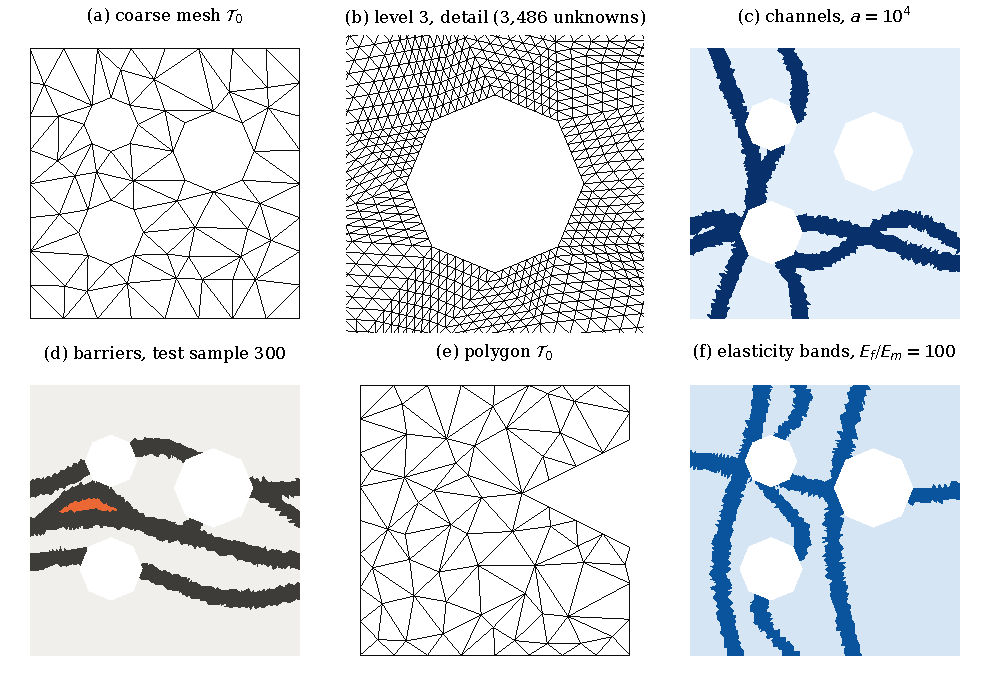
\includegraphics[width=0.92\linewidth]{figures/fig_setup.pdf}
\caption{Meshes and coefficient samples. (a) Unstructured coarse mesh $\mathcal{T}_0$ of the perforated square; (b) detail
of its third uniform refinement; (c) channels, conductive bands $a = 10^4$ (dark) in a unit background; (d) barriers,
insulating bands $a = 10^{-4}$ (dark), with a floating conductive island (orange, geometric label); (e) coarse mesh of the
polygonal domain; (f) elasticity, Young's modulus $100$ times larger in the bands. Field (c) is training sample 0 of held-out
data seed 1; field (d) is test sample 300 of the same seed, chosen as the first test sample whose floating island has more than
30 elements; (f) is training sample 0 of the elasticity data set.}\label{fig:setup}
\end{figure}

\paragraph{Data, training and metrics.} For each experiment 400 coefficient fields are drawn from the random seed $1000+s$,
where $s$ is the \emph{data seed}; samples $0$--$299$ train and $300$--$399$ test. Data seed $0$ was used during development;
all results are on the held-out data seeds $1$--$3$ unless stated otherwise. Each model is trained separately on each data
seed with network initialisation seed $0$; OA-VCB was in addition retrained with initialisation seeds $1$ and $2$
(Section~\ref{sec:initseeds}). All models share the same base loss (the mean of the relative $\ell^2$ and relative energy
errors of the predicted correction), AdamW with a one-cycle schedule (peak learning rate $2\times10^{-3}$), batch size 8 and
300 epochs; models with a Galerkin output add the same loss on their plain cycle output (Section~\ref{sec:output}). Every
learned model in the main comparisons has at most $22{,}000$ parameters (OA-VCB: 20{,}672); an equal cap and schedule do not
make the baselines equally well tuned, and no model was tuned per class. Training used NVIDIA T4 GPUs. The quantity of
interest is the algebraic error with respect to the discrete solution $u$ of $Au=F$, mainly in the energy norm,
$e = \|u - \hat u\|_A/\|u\|_A$; discretisation error is not part of any number. Comparisons are paired per test sample: for a
model and a reference,
\[
  G = \exp\Big(\tfrac1n\textstyle\sum_i \log\big(e^{\mathrm{ref}}_i/e^{\mathrm{model}}_i\big)\Big),\qquad
  W = \tfrac1n\#\{i: e^{\mathrm{model}}_i<e^{\mathrm{ref}}_i\},
\]
so $G>1$ favours the model. The 95\% intervals come from 5{,}000 paired bootstrap resamples of the test samples; they
describe variability over test operators for the trained models at hand, not over training runs. Arithmetic mean errors are
reported alongside; where the two summaries disagree we say so.

\paragraph{Use of generative AI in the research.} The software for this study (data generation, models, training and
evaluation, the classical comparators, the numerical checks of the propositions and the scripts that aggregate the stored
records into tables and figures) was written and run with the assistance of the generative AI system Claude (Anthropic),
under the author's direction; ChatGPT (OpenAI) was used to review the code, the results and the manuscript critically. No
reported number, table or data plot was produced by these tools directly: all are computed by the scripts from the stored
per-sample records (\appref{app:platform}), the principal summaries were recomputed by an independent script from the
per-sample arrays, and the structural properties of Section~\ref{sec:properties} were checked numerically by separate
scripts (\appref{app:impl}). Figure~\ref{fig:schematic} is TikZ source; no figure was created or edited with an image-generating
tool.

\paragraph{Classical comparators.} Next to every learned result we report, on the same samples and from the same $u_c$: the
classical reference of Section~\ref{sec:properties} (one deflated V$(4,4)$ cycle with degree-four Chebyshev smoothers on the
same transfers and Galerkin levels, with Galerkin output); the same cycle without deflation and projection; and two-grid
preconditioned conjugate gradients (weighted Jacobi$(1,1)$ smoothing and an exact level-$(L-1)$ Galerkin coarse solve). For
each test sample we record the first PCG iteration at which the energy error reaches OA-VCB's on that sample. The two
contained classical cycles of Proposition~\ref{prop:containment} are evaluated on the main test sets in \appref{app:impl}
(Table~\ref{tab:contained}): the fixed-interval Chebyshev member is as accurate as the reference to within a few per cent,
and the Jacobi member is $1.35$--$1.82$ times less accurate, so OA-VCB's margin over it is larger ($G = 15$--$16$ on channels,
$2.8$--$3.2$ on barriers).

\paragraph{Learned baselines.}\label{sec:baselines} For context we train learned operators of similar size under the same
protocol (\appref{app:baselines}): \emph{OA-Lift}, our earlier operator-adapted lifting network on the same hierarchy;
\emph{GNN}, a MeshGraphNet-type network; \emph{Transolver}; and Fourier, wavelet, lifting and multigrid neural operators
(FNO, WNO, LiNO, MgNO) on a uniform $63\times63$ grid. The suffix ``-op'' marks variants that receive the information of the
error equation (the scaled residual and, for graph models, the operator weights), like OA-VCB; every baseline starts from
$u_c$ and predicts only the correction. The grid models enter through a mesh--grid bridge whose handicap in the energy norm we
measure (\appref{app:bridge}), so their rows assess our adaptations in this setting, not those architectures on the
uniform-grid problems they were designed for. On the published Darcy benchmark (\appref{app:published}) a faithful FNO port
attains an error comparable to the published value and the official MgNO classes train successfully; these checks of the
implementations and of the benchmark pipeline do not validate every adaptation used in the unstructured-mesh experiments.

\subsection{Accuracy at four update stages}\label{sec:accuracy}\label{sec:channels}\label{sec:barriers}
\begin{table}[tbp]\centering\footnotesize\setlength{\tabcolsep}{4pt}
\caption{Main comparison, held-out data seeds 1--3 (100 test operators each; L3, $k_0=2$). Energy: mean of the three per-seed arithmetic mean relative energy errors. $G$: paired geometric-mean ratio of the classical reference's error to the model's over the pooled 300 samples [95\% CI]; $W$: fraction of samples on which the model is more accurate than the reference. All learned rows have 19{,}521--21{,}603 parameters. The other learned baselines (GNN, and the grid-based FNO-op, WNO-op, LiNO-op, MgNO, MgNO-op, which enter through a mesh--grid bridge) and further classical rows are in Tables~\ref{tab:channels} and~\ref{tab:barriers}.}\label{tab:core}
\begin{adjustbox}{max width=\linewidth}
\begin{tabular}{lllllll}\toprule
 & \multicolumn{3}{c}{channels (contrast $10^4$)} & \multicolumn{3}{c}{barriers (contrast $10^{-4}$)} \\ \cmidrule(lr){2-4}\cmidrule(lr){5-7}
model & energy & $G$ [95\% CI] & $W$ & energy & $G$ [95\% CI] & $W$ \\\midrule
OA-VCB (ours) & 2.75e-3 & 9.89 [9.57, 10.20] & 1.00 & 5.80e-2 & 2.00 [1.86, 2.14] & 0.88 \\
OA-VC (no deflation, plain output) & 3.46e-3 & 8.80 [8.45, 9.12] & 1.00 & 3.73e-1 & 0.61 [0.54, 0.70] & 0.43 \\
OA-Lift & 2.39e-2 & 1.06 [1.04, 1.09] & 0.63 & 3.52e-1 & 0.15 [0.14, 0.16] & 0.00 \\
GNN-op & 3.01e-2 & 0.84 [0.82, 0.86] & 0.19 & 3.61e-1 & 0.12 [0.11, 0.13] & 0.00 \\
Transolver-op & 1.85e-1 & 0.14 [0.13, 0.14] & 0.00 & 3.79e-1 & 0.11 [0.10, 0.12] & 0.00 \\
\midrule
classical reference (Chebyshev, $\nu=4$) & 2.57e-2 & 1 & -- & 8.11e-2 & 1 & -- \\
two-grid PCG, 6 iterations & 2.08e-3 & 14.13 [13.49, 14.81] & 1.00 & 5.05e-2 & 10.36 [8.76, 12.23] & 0.89 \\
$u_c$ alone & 3.73e-1 & 0.07 [0.07, 0.07] & 0.00 & 4.59e-1 & 0.07 [0.07, 0.08] & 0.00 \\
\bottomrule\end{tabular}
\end{adjustbox}
\end{table}

\begin{figure}[tbp]\centering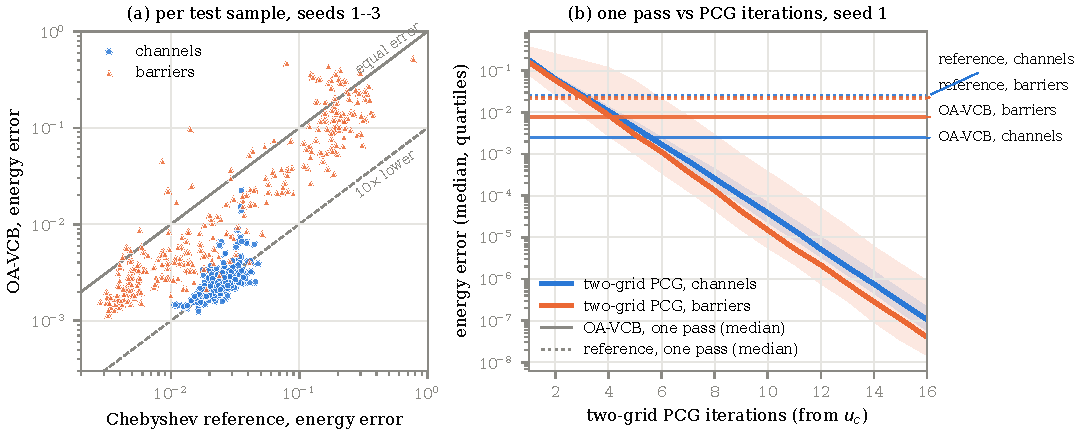
\includegraphics[width=\linewidth]{figures/fig_results.pdf}
\caption{(a) Energy error of OA-VCB against that of the Chebyshev reference on every test sample of held-out seeds 1--3
(300 channel and 300 barrier samples; points below the dashed line are more than ten times more accurate). (b) Energy error
of two-grid PCG from $u_c$ against the number of iterations (median, interquartile band; seed 1), with the median one-pass
errors of OA-VCB (solid) and of the reference (dotted).}\label{fig:results}
\end{figure}
\begin{figure}[tbp]\centering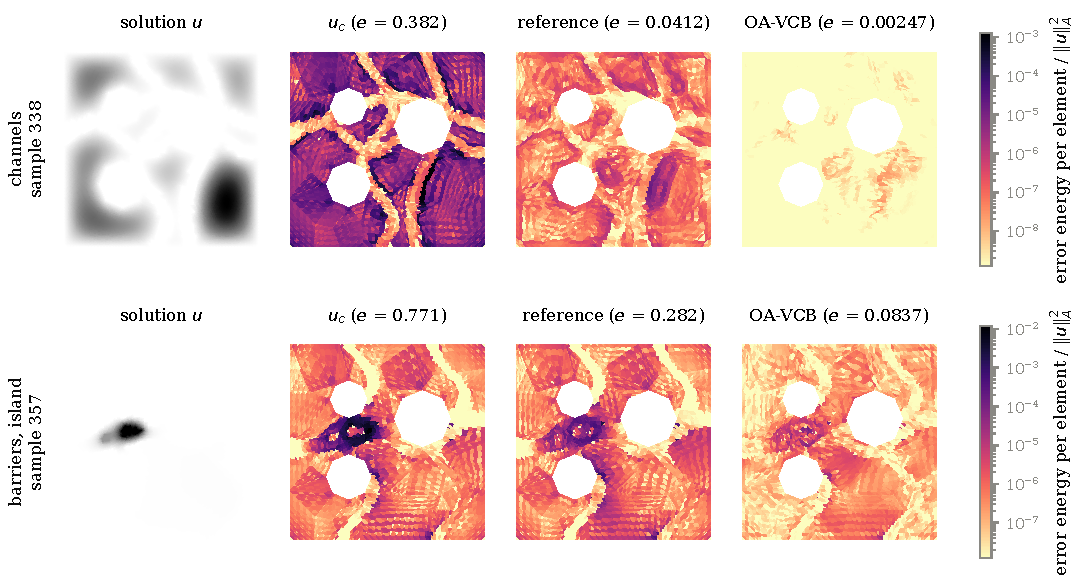
\includegraphics[width=\linewidth]{figures/fig_errormaps.pdf}
\caption{Solution and element-wise energy of the error, $a_e|\nabla(u-\hat u)|^2|T_e|/\|u\|_A^2$, for $\hat u = u_c$, the
Chebyshev reference and OA-VCB, on the median channel test sample (by OA-VCB error) and the median island sample of the
barriers (held-out seed 1). Shared logarithmic colour scale per row.}\label{fig:errormaps}
\end{figure}
\begin{table}[tbp]\centering\footnotesize\setlength{\tabcolsep}{4pt}
\caption{Barriers split by floating islands (geometric label, conductive component touching no Dirichlet node). Mean energy error OA-VCB / classical reference, paired $G$ and $W$ within each group, and OA-VCB's ratio of island to non-island mean error.}\label{tab:islands}
\begin{adjustbox}{max width=\linewidth}
\begin{tabular}{rrlllll}\toprule
seed & islands & with island & $G$, $W$ & without island & $G$, $W$ & ratio \\\midrule
1 & 39 & 0.100 / 0.167 & 1.86, 0.87 & 0.0075 / 0.0165 & 2.33, 0.95 & 13.4 \\
2 & 48 & 0.139 / 0.162 & 1.34, 0.67 & 0.0058 / 0.0140 & 2.70, 0.98 & 24.1 \\
3 & 40 & 0.143 / 0.188 & 1.56, 0.80 & 0.0056 / 0.0135 & 2.23, 0.95 & 25.6 \\
\bottomrule\end{tabular}
\end{adjustbox}
\end{table}

\paragraph{Channels.} OA-VCB is about ten times more accurate than its classical reference in the energy norm
(Table~\ref{tab:core}): $G = 10.23$, $9.76$ and $9.68$ on the three held-out seeds, and more accurate on every one of the 300
test samples (smallest per-sample ratio $1.57$; Figure~\ref{fig:results}(a)). Starting from the same $u_c$, two-grid PCG first
reaches OA-VCB's per-sample energy error after a median of $6$ iterations on each seed (range $5$--$8$;
Figure~\ref{fig:results}(b)). OA-VC, the same learned cycle without deflation and with the plain cycle output, is close
($G = 8.80$); on channels no near-kernel vectors are detected, so the two differ only in the output and its training term.
Among the learned baselines, OA-Lift is $6\%$ more accurate than the reference on average and the others are less accurate
(all nine in \appref{app:baselines}).

\paragraph{Barriers.} Barriers are harder for every method. OA-VCB's margin drops to $G = 2.13$, $1.93$, $1.93$ (pooled
$2.00$), and it is more accurate on $88\%$ of the samples. A minority of samples, those with floating islands, dominates
the mean (Table~\ref{tab:islands}): without islands OA-VCB is $2.2$--$2.7$ times more accurate than the reference, with mean
errors of $5.6$--$7.5\times10^{-3}$, comparable to channels; on island samples its mean error is $13$--$26$ times larger and its
margin shrinks to $G = 1.3$--$1.9$, with losses on $13$--$33\%$ of them. In Figure~\ref{fig:errormaps} the remaining error of
the median island sample is concentrated in and around the island. OA-VCB is never less accurate in energy than $u_c$, as
Proposition~\ref{prop:safeguard} guarantees, whereas OA-VC is less accurate than the reference ($G = 0.61$) and worse than
$u_c$ on $26$ of $300$ samples. Two-grid PCG first reaches OA-VCB's error after a median of $4$--$5$ iterations, with a range of
$2$--$14$ set by the island samples.

\paragraph{Repeated training.}\label{sec:initseeds} OA-VCB was retrained with two further initialisation seeds on every
held-out data set (\appref{app:repeat}, Table~\ref{tab:initseeds}). On channels the nine trained models give
$G = 9.68$--$10.74$, each with $W = 1$; the seed-0 models reported above are the least accurate of the three on every data
seed. On barriers $G = 1.80$--$2.13$ and $W = 0.83$--$0.94$, and the spread over initialisations on one data seed (at most
$0.13$ in $G$) is smaller than the spread over data seeds. These ranges describe training variability on the same test
operators, not independent test observations.

\subsection{The smoothing budget of the comparator}\label{sec:avt}
\begin{table}[tbp]\centering\footnotesize\setlength{\tabcolsep}{4pt}
\caption{Stronger classical smoothers and repeated classical passes, held-out seed 1, measured on one CPU (Intel(R) Xeon(R) Processor @ 2.80GHz, 2 threads; a different machine from Table~\ref{tab:cost}, so OA-VCB was re-timed): energy, the arithmetic mean relative energy error over the 100 test samples (the quantity plotted in Figure~\ref{fig:avt}); $G$, the paired geometric-mean ratio of each classical variant's error to OA-VCB's [95\% CI] (below 1: the classical variant is more accurate in this metric); $W$, the fraction of samples on which OA-VCB is more accurate; and the mean time per sample from $u_c$ with set-up, in ms (classical rows: per-sample minimum over the repetitions; OA-VCB: operator data and batched inference, minimum over the repetitions of the whole-test-set time divided by the number of samples). The eight- and sixteen-step rows exceed the residual-polynomial degree covered by Proposition~\ref{prop:containment} for the four-stage architecture; no learned model with that larger budget was trained.}\label{tab:avt}
\begin{adjustbox}{max width=\linewidth}
\begin{tabular}{lllll}\toprule
method & energy & $G$ [95\% CI] & $W$ & ms \\\midrule
\multicolumn{5}{l}{\emph{channels}: OA-VCB 2.55e-3, 268\,ms} \\
\quad reference, Chebyshev $\nu=4$ (Table~\ref{tab:core}) & 2.59e-2 & 10.23 [9.75, 10.71] & 1.00 & 83 \\
\quad reference, Chebyshev $\nu=8$ & 1.08e-2 & 4.23 [4.00, 4.46] & 1.00 & 79 \\
\quad reference, Chebyshev $\nu=16$ & 4.72e-3 & 1.83 [1.73, 1.93] & 0.99 & 85 \\
\quad reference, symmetric Gauss--Seidel, 4 sweeps & 2.06e-2 & 8.10 [7.69, 8.49] & 1.00 & 77 \\
\quad reference ($\nu=4$) applied twice & 3.50e-3 & 1.30 [1.21, 1.40] & 0.79 & 87 \\
\quad reference ($\nu=4$) applied 3 times & 5.51e-4 & 0.19 [0.17, 0.21] & 0.00 & 88 \\
\multicolumn{5}{l}{\emph{barriers}: OA-VCB 4.36e-2, 273\,ms} \\
\quad reference, Chebyshev $\nu=4$ (Table~\ref{tab:core}) & 7.51e-2 & 2.13 [1.90, 2.38] & 0.92 & 80 \\
\quad reference, Chebyshev $\nu=8$ & 6.47e-2 & 1.25 [1.09, 1.42] & 0.64 & 83 \\
\quad reference, Chebyshev $\nu=16$ & 5.87e-2 & 0.82 [0.69, 0.97] & 0.45 & 85 \\
\quad reference, symmetric Gauss--Seidel, 4 sweeps & 7.30e-2 & 2.11 [1.87, 2.36] & 0.92 & 80 \\
\quad reference ($\nu=4$) applied twice & 2.66e-2 & 0.29 [0.24, 0.35] & 0.13 & 84 \\
\quad reference ($\nu=4$) applied 3 times & 1.21e-2 & 0.05 [0.03, 0.06] & 0.02 & 88 \\
\bottomrule\end{tabular}
\end{adjustbox}
\end{table}

\begin{figure}[tbp]\centering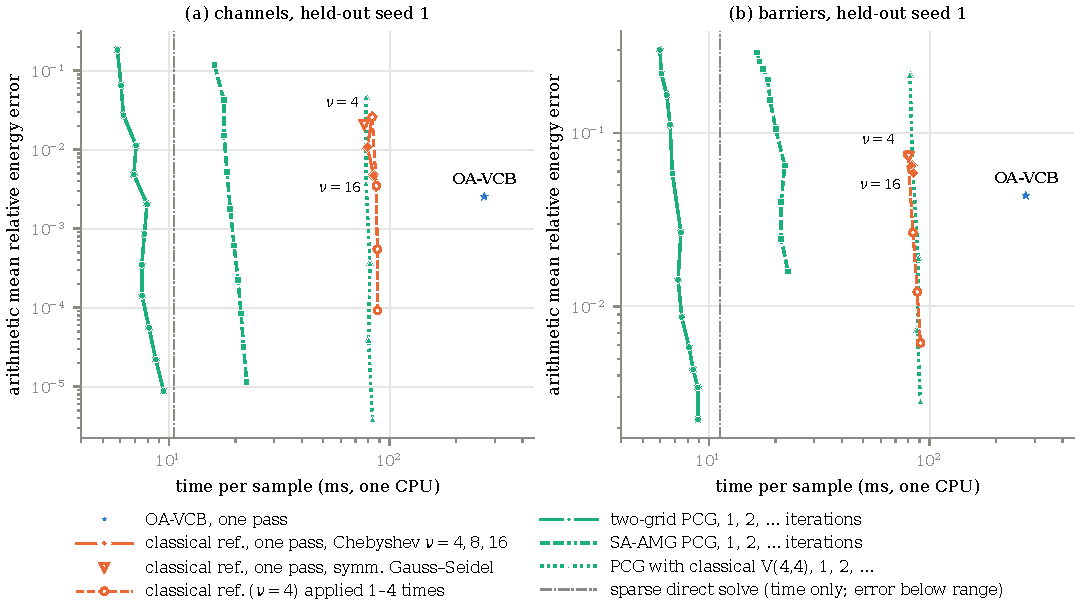
\includegraphics[width=\linewidth]{figures/fig_avt.pdf}
\caption{Arithmetic mean relative energy error against mean time per sample from $u_c$, set-up included, held-out seed 1, all
methods measured in one run on one CPU (Table~\ref{tab:avt}; the paired $G$ of the table is a different summary). Classical
reference: one pass with Chebyshev smoothing of degree $\nu=4$, $8$, $16$ or symmetric Gauss--Seidel, and the $\nu=4$ reference
applied one to four times. PCG curves: one point per iteration. The vertical line marks only the time of the sparse direct
solve, whose error is at solver accuracy, below the plotted range.}\label{fig:avt}
\end{figure}
The margins above compare four learned update stages per pre- and post-smoother with a degree-four Chebyshev reference.
Table~\ref{tab:avt} and Figure~\ref{fig:avt} vary the classical smoothing budget on held-out seed 1, with every method, OA-VCB
included, timed in one run on one machine (\appref{app:platform}). On channels the paired margin falls from $10.2$ at $\nu=4$ to
$4.2$ at $\nu=8$ and $1.8$ at $\nu=16$ ($W = 0.99$). On barriers, sixteen-step Chebyshev reverses the advantage by the paired
geometric-mean metric ($G = 0.82$, with the classical pass more accurate on $55$ of $100$ samples), although OA-VCB retains the
smaller arithmetic mean error ($0.0436$ against $0.0587$). Symmetric Gauss--Seidel with four sweeps is close to the $\nu=4$
reference ($G = 8.1$ and $2.1$). Repeated classical passes give the stronger practical conclusion. Applying the $\nu=4$
reference twice brings it within a paired factor $1.30$ of OA-VCB on channels and makes it $3.5$ times more accurate on barriers
(paired geometric gains; on barriers the mean error is lower as well, $0.0266$); three applications are $5.3$ and $22$ times more
accurate by the paired metric and have lower mean errors on both families ($5.5\times10^{-4}$ and $0.0121$). Because the
operator-adapted hierarchy dominates the classical set-up, every classical variant takes $77$--$88$\,ms per sample, against
$268$--$273$\,ms for OA-VCB on this machine. The eight- and sixteen-step comparisons exceed the residual-polynomial degree
covered by Proposition~\ref{prop:containment} for the four-stage architecture. They test a larger classical smoothing budget; no
learned model with that larger budget was trained. The one-pass margins therefore measure what learning adds at a fixed number
of update stages; at equal cost, on these measurements, the learned pass is not the more accurate one.

\subsection{Cost at matched accuracy}\label{sec:cost}
\begin{table}[tbp]\centering\footnotesize\setlength{\tabcolsep}{4pt}
\caption{Cost per test sample on one CPU (2 threads), channels, held-out seed 1, in ms. Every row starts from the assembled fine matrix; its assembly (1.4 / 5.4 ms, common to all methods) is not included. Per-operator set-up is included in every row; the sparsity patterns of the hierarchy, computed once per mesh (71 / 871 ms), and training are not. Classical rows: mean over the 100 samples of the per-sample minimum over 3 (L3) / 2 (L4) repetitions; OA-VCB operator data and inference: minimum over the repetitions of the whole-test-set time divided by 100. Iteration counts were determined beforehand, untimed, with the reference solution (a matched-accuracy benchmark, not a stopping criterion).}\label{tab:cost}
\begin{adjustbox}{max width=\linewidth}
\begin{tabular}{lll}\toprule
 & L3, $k_0=2$ (3{,}486 unknowns) & L4, $k_0=3$ (14{,}398) \\\midrule
\multicolumn{3}{l}{\emph{OA-VCB (one pass)}} \\
$u_c$ (level-$k_0$ Galerkin factor and solve) & 2.1 & 9.6 \\
operator data (hierarchy, Galerkin levels, $Z$) & 66.6 & 841.3 \\
inference, batch 8 (batch 1) & 96.0 (176.7) & 1{,}561.0 (1{,}461.8) \\
\textbf{total} (batch 8) & 164.8 & 2{,}411.8 \\
\midrule\multicolumn{3}{l}{\emph{single classical pass, error not matched (10 times larger)}} \\
classical reference, from $u_c$ & 60.1 & 769.1 \\
\midrule\multicolumn{3}{l}{\emph{iterative, run to OA-VCB's error on each sample [median; range of iterations]}} \\
two-grid PCG & 5.7 [6; 5--7] & 24.7 [6; 4--8] \\
SA-AMG PCG & 13.5 [5; 4--6] & 41.5 [6; 4--7] \\
PCG with the classical V(4,4) & 61.2 [3; 2--3] & 794.1 [3; 2--3] \\
\midrule\multicolumn{3}{l}{\emph{direct, to solver accuracy}} \\
sparse direct solve (SuperLU) & 8.2 & 48.1 \\
\bottomrule\end{tabular}
\end{adjustbox}
\end{table}

Table~\ref{tab:cost} compares the cost per sample on one CPU of a second machine (\appref{app:platform}). Every row starts
from the assembled fine matrix and includes per-operator set-up; the once-per-mesh sparsity patterns and training are not
included. The iterative methods run, on each sample, exactly the number of iterations that reaches OA-VCB's energy error there;
these counts were determined beforehand with the reference solution, outside the timing, so this is a matched-accuracy
benchmark rather than a deployable stopping rule. Two-grid PCG, SA-AMG PCG and a sparse direct solve are far cheaper than
OA-VCB: at L3, $5.7$, $13.5$ and $8.2$\,ms against $165$\,ms, factors of $29$, $12$ and $20$; at L4 the factors grow to $98$, $58$ and
$50$. The direct solve reaches solver accuracy, much higher than OA-VCB's. From L3 to L4 (4.1 times the unknowns) OA-VCB's time
grows by a factor $15$ and two-grid PCG's by $4.3$. Two components dominate. The operator-adapted hierarchy takes $52$ of the
$67$\,ms of operator data at L3 and $722$ of $841$\,ms at L4; it is a cost of the adapted transfers and their growing operator
complexity, shared with the classical reference, not a cost of learning. The network's CPU inference alone is $17$ (L3) and
$63$ (L4) times the full two-grid PCG time including its set-up, so amortising training over repeated solves cannot make the
learned pass the cheaper route on these configurations. As context only, on the T4 GPU used for training, inference took
$13$\,ms per sample at L3 in batches of eight; optimised implementations, batched GPU operator data and reuse of an operator
for many right-hand sides were not measured.

% Sections 5-6 -- design ablations; limitations and robustness.  v3, 13 Oct 2026 (FINAL_SUBMISSION_REVIEW_ASTRA: compressed;
% protocol details, per-seed tables and the extensions moved to the appendix).
\section{What the learned cycle gains: design ablations}\label{sec:design}

\subsection{Deflation, output and non-linearity}\label{sec:ablation}
\begin{table}[tbp]\centering\footnotesize\setlength{\tabcolsep}{4pt}
\caption{Separately trained design variants, held-out data seed 1. Deflation, output used at inference (plain cycle or Galerkin projection), training loss and smoother class; mean energy error with each model's own output and reference/model $G$, $W$. OA-VCQ was not run on channels, where no near-kernel vectors are detected.}\label{tab:factorial}
\begin{adjustbox}{max width=\linewidth}
\begin{tabular}{llllllllll}\toprule
 & deflation & output & loss & smoothers & params & \multicolumn{2}{c}{barriers: energy, ($G$, $W$)} & \multicolumn{2}{c}{channels: energy, ($G$, $W$)} \\\midrule
OA-VC & no & plain & plain & learned & 20{,}672 & 2.33e-1 & 0.71, 0.44 & 4.08e-3 & 8.83, 0.99 \\
OA-VCZ & yes & plain & plain & learned & 20{,}672 & 7.51e-2 & 1.52, 0.75 & 3.52e-3 & 8.72, 0.99 \\
OA-VCQ & no & Galerkin & plain + proj. & learned & 20{,}672 & 1.07e-1 & 1.15, 0.65 & -- & -- \\
OA-VCB & yes & Galerkin & plain + proj. & learned & 20{,}672 & 4.36e-2 & 2.13, 0.92 & 2.55e-3 & 10.23, 1.00 \\
OA-VCL & yes & plain & plain & residual-linear & 21{,}600 & 1.51e-1 & 0.70, 0.16 & 1.11e-2 & 2.59, 0.97 \\
OA-VCBL & yes & Galerkin & plain + proj. & residual-linear & 21{,}600 & 6.76e-2 & 1.13, 0.69 & 1.01e-2 & 2.72, 0.99 \\
\bottomrule\end{tabular}
\end{adjustbox}
\end{table}

Table~\ref{tab:factorial} compares separately trained design variants on held-out seed 1; \appref{app:repeat} evaluates each
trained network with both outputs, plain and projected (Table~\ref{tab:factorial8}). Except for the residual-linear channel
control, each comparison rests on one initialisation seed per model.
\emph{Deflation.} On barriers, adding indicator deflation improves the paired accuracy by $G = 2.14$ with plain output
(OA-VC $\to$ OA-VCZ) and by $1.85$ with Galerkin output (OA-VCQ $\to$ OA-VCB). Without it no variant beats the reference by more
than $15\%$. On channels deflation is inactive.
\emph{Galerkin output and its training term.} On barriers the Galerkin output with the additional loss term adds $G = 1.63$
without deflation (OA-VC $\to$ OA-VCQ) and $1.40$ with it (OA-VCZ $\to$ OA-VCB); on channels OA-VCB is $1.17$ times more accurate
than OA-VCZ. The two components interact: without deflation, training for the projected output improves the projected output
($0.121\to0.107$) but degrades the plain one ($0.233\to0.311$); with deflation both improve ($0.049\to0.044$ projected,
$0.075\to0.066$ plain). The gains are therefore not independent and additive.
\emph{Non-linearity.} The non-linear learned smoothers outperform the tested residual-linear controls, which keep the same
operator-dependent structure but make the smoother maps linear in their right-hand side (OA-VCL is linear in $r$ for each
$A$; OA-VCBL's Galerkin output is not). On channels the residual-linear models still gain over the Chebyshev reference
($G = 2.59$ for OA-VCL, $2.72$ for OA-VCBL), and the non-linear smoothers add a further $3.36$ (plain output) and $3.76$ (Galerkin
output); on barriers the residual-linear models gain little or lose ($G = 1.13$ and $0.70$), and non-linearity adds $1.9$--$2.2$.
The product $2.72\times3.76 = 10.2$ follows algebraically from chaining paired geometric-mean ratios; it is not a causal
decomposition. Over three initialisation seeds of OA-VCBL the two factors are $2.63$--$2.72$ and $3.76$--$4.08$ (OA-VCB of the
same seed index). One OA-VCBL run (seed 2) ended with a different optimisation outcome, a $2.8$ times higher final training loss
and a plain-cycle error of $5.9\times10^{-2}$ instead of $1.07\times10^{-2}$, while its projected mean error is similar
($9.8\times10^{-3}$ against $1.01\times10^{-2}$; its paired gain is slightly lower, $2.63$): projected accuracy is stable despite
the sensitivity of the plain cycle and of the training objective.

\subsection{Operator-adapted transfers}\label{sec:transfers}
\begin{table}[tbp]\centering\footnotesize\setlength{\tabcolsep}{4pt}
\caption{Operator-adapted ($m=4$) vs geometric ($m=0$) transfers, separately trained OA-VCB models on the same data. OA-VCB error with each; paired $G$ (geometric-transfer error / adapted-transfer error) and $W$; the same ratio for the two classical references; and reference/learned $G$ for each choice of transfers.}\label{tab:transfers}
\begin{adjustbox}{max width=\linewidth}
\begin{tabular}{llllllll}\toprule
case & adapted & geometric & $G$ geom./adapt. & $W$ & references: geom./adapt. & reference/learned (adapt.) & reference/learned (geom.) \\\midrule
channels, seed 1 & 2.55e-3 & 5.02e-3 & 1.91 [1.84, 2.00] & 1.00 & 1.24 & 10.23 & 6.65 \\
channels, seed 2 & 2.79e-3 & 5.46e-3 & 1.92 [1.84, 2.00] & 1.00 & 1.24 & 9.76 & 6.30 \\
channels, seed 3 & 2.92e-3 & 5.66e-3 & 1.87 [1.80, 1.95] & 1.00 & 1.25 & 9.68 & 6.50 \\
barriers, seed 1 & 4.36e-2 & 1.13e-1 & 4.07 [3.50, 4.71] & 0.97 & 2.82 & 2.13 & 1.48 \\
\bottomrule\end{tabular}
\end{adjustbox}
\end{table}

To isolate the operator-adapted transfers, OA-VCB was retrained with $m=0$ in \eqref{eq:jacobi} (the geometric prolongation)
on the same data (Table~\ref{tab:transfers}). The adapted transfers make the learned cycle $1.9$ times more accurate on
channels, on every sample of all three seeds, and $4.1$ times more accurate on barriers ($97\%$ of samples). They help the
learned cycle more than the classical one ($1.24$ and $2.82$ for the references), and the margin of learning over the classical
reference is larger with them ($10.2$ against $6.7$ on channels, seed 1; $2.13$ against $1.48$ on barriers). Because the two
models are trained separately, the comparison measures the choice of transfers under our training protocol, including its
effect on optimisation. The adapted transfers are also more expensive: operator data $121$--$152$ instead of $11$--$14$\,ms per
sample on the training platform's CPU. Retraining with $m = 8$ keeps the margin over the correspondingly stronger reference
($G = 11.17$ on channels, $2.01$ on barriers; \appref{app:sensitivity}), so it is not an artefact of the cheaper transfers.

\section{Limitations and robustness}\label{sec:failure}

\subsection{Floating islands}\label{sec:islands}
Floating islands are present in $39$--$48\%$ of the barrier test samples, and island samples have larger mean energy errors
for every method tested (Table~\ref{tab:islands}). Indicator deflation improves the tested barrier models
(Section~\ref{sec:ablation}), while OA-VCB's remaining island errors ($0.10$--$0.14$) are still large. An island indicator is
constant on the island, whereas the low-energy mode it approximates also varies across the surrounding barrier. We therefore
asked, with a protocol fixed in writing before any number was computed (\appref{app:harmonic}), how much of OA-VCB's remaining
error lies in $A$-harmonic extensions of the indicators into a patch of $\rho = 2$ graph rings, added as a sequential
$A$-orthogonal correction of the frozen prediction; the outcome was decided on $100$ fresh coefficient fields per checkpoint.
On the 89 detector-positive fresh operators, the correction reduces OA-VCB's mean energy error from $0.1219$ to $0.1043$
($R = 14.4\%$, paired 95\% interval $9.8$--$19.5\%$; Table~\ref{tab:harmonic}) and outperforms a patch-indicator control of
equal support by a paired factor $1.13$, but it does not meet the prespecified support threshold: the outcome is ``little
support from the tested enrichment''. On a fixed 40-sample subset, extending the basis globally raises the reduction from
$10.9\%$ to $20.9\%$, so localisation matters, but substantial error remains. After the same correction is applied to both,
OA-VCB keeps its advantage over the reference on island samples ($G = 1.42$ [1.27, 1.60]). These results concern sequential
post-processing of frozen predictions; they do not assess an enlarged output space or retraining with enriched deflation.

\subsection{Dependence on the load}\label{sec:rhs}
\begin{table}[tbp]\centering\footnotesize\setlength{\tabcolsep}{4pt}
\caption{Load dependence (channels, held-out data seeds 1--3, the same 300 operators for every load; $u_c$ recomputed for each load). Pooled reference/OA-VCB $G$ [95\% CI] and $W$ for the models trained with the single load $f=1$ and for the models trained on the random-load distribution (one model per data seed; $W$: smallest of the three per-seed win fractions), and the paired ratio of the fixed-load models' error to the random-load models' (above 1 favours the random-load models). Per-seed values and mean errors: Tables~\ref{tab:rhs} and~\ref{tab:rhsrandom}.}\label{tab:loads}
\begin{adjustbox}{max width=\linewidth}
\begin{tabular}{llllll}\toprule
load & fixed-load $G$ [95\% CI] & $W$ & random-load $G$ [95\% CI] & $W$ (min) & fixed/random \\\midrule
$f=1$ & 9.89 [9.57, 10.20] & 1.00 & 6.87 [6.62, 7.13] & 1.00 & 0.70 \\
$f=-1$ & 0.21 [0.20, 0.23] & 0.00 & 6.51 [6.27, 6.75] & 1.00 & 30.8 \\
$f=3$ (homogeneity check) & 9.89 [9.57, 10.20] & 1.00 & 6.87 [6.62, 7.13] & 1.00 & 0.70 \\
random-load distribution (Sec.~\ref{sec:k0}) & 0.60 [0.50, 0.72] & 0.37 & 6.22 [5.99, 6.44] & 1.00 & 10.3 \\
smooth, both signs & 0.20 [0.19, 0.23] & 0.06 & 6.38 [6.20, 6.56] & 1.00 & 31.1 \\
localised source & 0.44 [0.38, 0.51] & 0.32 & 2.51 [2.25, 2.79] & 0.79 & 5.7 \\
\bottomrule\end{tabular}
\end{adjustbox}
\end{table}

The models of Section~\ref{sec:accuracy} were trained with the single load $f=1$ and approximate the fixed-load map
$a\mapsto u(a;f)$. Table~\ref{tab:loads} applies them and the models trained on a load distribution (Section~\ref{sec:k0}) to
other loads on the same test operators. Positive scaling ($f=3$) reproduces the relative errors of $f=1$, as
Proposition~\ref{prop:homogeneity} guarantees. The other tested load families reverse the fixed-load models' advantage: with
$f=-1$ OA-VCB is less accurate than the reference on all 300 operators ($G = 0.21$), and for smooth loads of both signs,
localised sources and the random-load distribution the reference is more accurate as well ($G = 0.20$--$0.60$). The energy
safeguard holds throughout (never worse than $u_c$ on the $1{,}800$ load--sample pairs) and shows what it promises: no damage,
not accuracy. Training on the load distribution changes this: the random-load models are more accurate than the reference by
$G = 6.2$--$6.9$ on $f=\pm1$, smooth loads and held-out random loads, with $W = 1$ on every seed, at the price of a $1.44$-fold
loss on $f=1$ against fixed-load training. On pure localised sources the pooled gain is $2.51$, but the per-seed win fractions
are $0.89$, $0.79$ and $0.83$, so the criterion fixed before this test ($G\ge2$ and $W\ge0.8$ per seed) is missed on seed 2, by one
sample. These tests support broader forcing coverage after distributional training; they do not establish arbitrary-load
accuracy (load definitions and per-seed values in \appref{app:loads}).

\subsection{Further settings}\label{sec:k0}\label{sec:l4}\label{sec:aniso}
\begin{table}[tbp]\centering\footnotesize\setlength{\tabcolsep}{4pt}
\caption{Further settings: mean energy error of OA-VCB and of its classical reference, paired reference/OA-VCB $G$ [95\% CI] and $W$, and the per-sample number of two-grid PCG iterations, from the same starting point, at which PCG first reaches OA-VCB's energy error (median, range; computed iteration histories: 12 for $k_0=0$, 16 otherwise).}\label{tab:settings}
\begin{adjustbox}{max width=\linewidth}
\begin{tabular}{llllll}\toprule
setting & OA-VCB & reference & $G$ [95\% CI] & $W$ & PCG its \\\midrule
$k_0=0$ (no external coarse solution), seed 1 & 7.62e-3 & 8.52e-2 & 11.39 [10.95, 11.83] & 1.00 & 5 (4--7) \\
$k_0=0$ (no external coarse solution), seed 2 & 7.58e-3 & 8.04e-2 & 10.91 [10.35, 11.44] & 1.00 & 5 (4--6) \\
$k_0=0$ (no external coarse solution), seed 3 & 8.13e-3 & 8.55e-2 & 10.82 [10.40, 11.26] & 1.00 & 5 (5--7) \\
finer hierarchy (L4, $k_0=3$), seed 1 & 2.21e-3 & 2.01e-2 & 9.72 [9.04, 10.33] & 1.00 & 6 (4--8) \\
polygonal domain, seed 1 & 3.54e-3 & 3.30e-2 & 9.39 [8.89, 9.86] & 1.00 & 6 (5--8) \\
random loads (in distribution), seed 1 & 4.50e-3 & 2.65e-2 & 6.27 [5.89, 6.65] & 1.00 & 5 (4--7) \\
random loads (in distribution), seed 2 & 4.26e-3 & 2.51e-2 & 6.05 [5.72, 6.36] & 1.00 & 5 (4--7) \\
random loads (in distribution), seed 3 & 4.54e-3 & 2.61e-2 & 6.34 [5.90, 6.77] & 1.00 & 6 (4--7) \\
anisotropic tensor coefficient, seed 0 (dev.) & 6.21e-3 & 2.10e-2 & 3.50 [3.33, 3.68] & 1.00 & -- \\
anisotropic tensor coefficient, seed 1 & 6.01e-3 & 2.04e-2 & 3.51 [3.33, 3.69] & 1.00 & -- \\
anisotropic tensor coefficient, seed 2 & 6.17e-3 & 2.12e-2 & 3.58 [3.40, 3.77] & 1.00 & -- \\
\bottomrule\end{tabular}
\end{adjustbox}
\end{table}

Table~\ref{tab:settings} summarises separately trained variations of the main configuration (details in
\appref{app:settings}). Without an externally supplied coarse solution ($k_0=0$; the cycle still contains its exact 28-node
coarsest solve) OA-VCB keeps $G = 10.8$--$11.4$ with $W = 1$, and the energy safeguard then only bounds the damage relative to
$u=0$. A separately trained finer hierarchy ($L=4$, 14{,}398 unknowns) gives $G = 9.72$, a polygonal domain $9.39$, an anisotropic
tensor coefficient $3.5$--$3.6$, and training and testing on the random-load distribution $6.05$--$6.34$, all with $W=1$.
\emph{Refinement without retraining.} The L4-trained model applied unchanged to the next refined mesh (L5, 58{,}494 unknowns,
100 test samples) keeps $G = 8.12$ [7.50, 8.67] with $W = 1$, a per-sample gain $0.84$ [0.76, 0.91] times that at L4 on the same
coefficient draws. At L6 (235{,}774 unknowns) the evaluation was stopped by the platform's session limit after 21 of 24 planned
samples; on these completed cases $G = 4.18$ [3.43, 4.88] with $W = 1$, about half the L5 gain on the same draws. This partial
evaluation shows a retained but shrinking margin; it does not establish mesh independence, and the coarse level, the bottom
level of the cycle and the distance from the training mesh change together. A model trained at L3 does not keep its margin at
L4 ($G = 1.95$ on 20 samples). \emph{Plane-strain elasticity} (one data set, one training run; preliminary): without deflation and without
tuning, OA-VCB is more accurate than its Chebyshev reference on every test sample ($G = 2.32$; \appref{app:settings}).

% Sections 7-8 -- discussion and conclusion.  v3, 13 Oct 2026 (FINAL_SUBMISSION_REVIEW_ASTRA: four focused paragraphs; old
% flexible-CG pilot removed; speculative uses reduced to one sentence; design lessons narrowed; conclusion ~180 words).
\section{Discussion}\label{sec:discussion}

\paragraph{What is learned, and what the control shows.} The classical reference receives the same transfers, Galerkin
levels, coarse solution, deflation vectors and output projection as OA-VCB, and the contained fixed-interval Chebyshev member
is within a few per cent of it, so the margins of Section~\ref{sec:accuracy} measure what four learned update stages per
smoother add to one pass through this cycle. That contribution is reproducible across data seeds and training
initialisations, and the ablations locate parts of it under this training protocol: the adapted hierarchy materially improves
the learned cycle (the direct comparison with geometric transfers gives $1.9$ on channels and $4.1$ on barriers), learning
already helps within the residual-linear class ($2.6$--$2.7$ on channels), and the nonlinearity adds a further $3.4$--$3.8$.
The baseline tables of \appref{app:baselines} are supporting context, not evidence for this attribution. The comparison does
not show that the learned pass approximates $A^{-1}$ in any uniform sense.

\paragraph{Why the one-pass advantage does not buy a solver advantage.} Equal update count is a controlled architectural
comparison, not equal work. Additional classical smoothing is cheap on the operator-adapted hierarchy, and with it the margin
falls to $1.8$ on channels and reverses on barriers by the paired metric; three classical passes are more accurate than the
learned pass on both families at about a third of its time (Section~\ref{sec:avt}). Against converged-to-target solvers the gap is one to two
orders of magnitude and grows with the mesh (Section~\ref{sec:cost}); because the network inference alone exceeds a complete
two-grid PCG solve including its set-up, no number of repeated solves amortises training on the tested configurations.
Operator reuse across many right-hand sides and batched GPU execution remain untested and would have to be measured against
equally optimised classical implementations; a correction that is nonlinear in the load would also need a suitable outer
method if used inside an iteration. The operator complexity of the hierarchy ($4.5$ for three levels, $8.6$ for four) would
limit the approach in three dimensions or with more levels unless the prolongations are truncated, as in smoothed aggregation
\cite{vanek1996}, which was not tested.

\paragraph{Loads and floating islands.} The network is positively homogeneous but not linear in the residual. Trained with
one load, it learns corrections for the residuals that this load produces and loses or reverses its advantage on others;
training on a load distribution restores a six-fold margin on that distribution and on smooth loads of both signs, and a
smaller, less uniform one for localised sources (Section~\ref{sec:rhs}). A correction linear in the residual for each fixed
operator would enforce superposition and sign symmetry but would not by itself guarantee accuracy on unseen load directions,
and the tested residual-linear smoothers recover only part of the gain. Indicator deflation improves the tested barrier
models, while substantial error remains on island samples. The tested sequential harmonic enrichment removes only a modest
part of that error; richer coarse spaces, for example contrast-robust spaces built from local spectral problems
\cite{galvis2010,spillane2014geneo,chung2018cem,ma2022} or learned ones \cite{rudikov2025lsino}, are one plausible
continuation, not a remedy established here.

\paragraph{Implications for learned multilevel components.} Four observations bear on how learned components of
multigrid methods are evaluated, beyond the tested implementation. First, a margin measured at one classical smoothing budget
can overstate what learning adds: on the same hierarchy the paired margin fell from $10.2$ to $4.2$ and $1.8$ on channels, and
from $2.1$ to $1.25$ and $0.82$ on barriers, as the Chebyshev degree rose from four to eight and sixteen
(Section~\ref{sec:avt}), so learned smoothers should be compared across that budget. Second, the hierarchy and the learning
interact, and should be varied separately: with geometric transfers the learned cycle was $1.9$ and $4.1$ times less
accurate, and its margin over the classical reference on the same transfers was also smaller ($6.3$--$6.7$ instead of
$9.7$--$10.2$ on channels, $1.48$ instead of $2.13$ on barriers; Table~\ref{tab:transfers}), so in this study the learned
smoothers gained more on the operator-adapted hierarchy than on the geometric one. Third, averages hide where a learned cycle
fails: the error that remained on floating islands after learned smoothing and indicator deflation is visible only when those
samples are reported separately (Section~\ref{sec:islands}). Fourth, a smoother that is nonlinear in the residual is trained
for the residuals of its training loads, so those loads have to sample the loads of the intended use
(Section~\ref{sec:rhs}). Finally, a one-pass accuracy gain at an equal update count does not by itself establish a
computational benefit; that has to be shown at matched accuracy and cost (Section~\ref{sec:cost}).

\paragraph{Scope.} All experiments are two-dimensional with $P_1$ elements; coefficient contrasts are $10^4$ for the
isotropic families, tow coefficients $100$ and $5$ against a unit background for the anisotropic case and a stiffness ratio
of $100$ for the preliminary elasticity case; one family of perforated domains and one polygon are used; models were trained
on meshes of at most 14{,}398 unknowns, and one was applied without retraining to meshes of up to 235{,}774 unknowns, where its
margin shrinks. The learned baselines are adaptations of published architectures to this setting.

\section{Conclusion}\label{sec:conclusion}
We asked what learned smoothing adds to one pass of a multigrid cycle whose transfers, coarse operators, coarsest solve and
deflation vectors are computed from each operator. With four update stages per smoother, the learned pass is about ten times
more accurate in the energy norm than a degree-four Chebyshev-smoothed pass on the same hierarchy for conductive channels and
about twice as accurate for insulating barriers, reproducibly across data seeds and training runs, and the adapted transfers,
deflation, Galerkin output and nonlinearity each contribute. The same experiments bound the result. The margin shrinks quickly
when the classical pass receives more smoothing, and three classical passes are more accurate at a third of the cost; the advantage
depends on the training load; floating islands keep substantial error; and the implementation is much slower than converged
classical solvers at matched accuracy. Learned smoothing is therefore a measurable source of accuracy within a prescribed
multilevel pass, not yet a practical solver. The open challenge is a workload, and an implementation, in which that accuracy
lowers the total cost of reaching a required tolerance.


% Declarations.  13 Oct 2026; 13 Oct (pm): code and data on request (author's decision); AI declaration per Elsevier policy of Aug 2026.  Funding and competing interests as stated by the author (13 Oct); AI tools as named by the
% author (Claude, ChatGPT).
\section*{CRediT authorship contribution statement}
\textbf{Kumar Kaushik Ranjan:} Conceptualization, Methodology, Software, Validation, Formal analysis, Investigation, Data
curation, Writing -- original draft, Writing -- review \& editing, Visualization.

\section*{Declaration of competing interest}
The author declares no known competing financial interests or personal relationships that could have appeared to
influence the work reported in this paper.

\section*{Funding}
This research did not receive any specific grant from funding agencies in the public, commercial, or not-for-profit sectors.

\section*{Declaration of generative AI and AI-assisted technologies in the manuscript preparation process}
During the preparation of this work the author used Claude (Anthropic) in order to draft and edit the manuscript text and to
assemble its tables and figures from the stored results, and ChatGPT (OpenAI) in order to review the manuscript critically.
The use of these tools in the research itself is described in Section~\ref{sec:protocol}. After using these tools, the author
reviewed and edited the content as needed and takes full responsibility for the content of the published article.

\section*{Code and data availability}
The source code (data generation, models, training and evaluation, identified by the hash \texttt{f8653612eb84} stored with
every result), the raw per-sample result records, the trained checkpoints and the scripts that regenerate every table and
figure from the records will be made available by the corresponding author on reasonable request.

% Appendix (supplementary material).  v2, 13 Oct 2026 (FINAL_SUBMISSION_REVIEW_ASTRA: implementation details, full baseline
% tables, per-seed tables, protocols and extensions moved here from the main text; Session-9 scope corrected).
% Tables generated by manuscript/make_tables.py (except tab_related, hand-written).
\clearpage
\appendix
\section{Contained classical cycles, implementation details and numerical checks}\label{app:impl}
\begin{table}[tbp]\centering\footnotesize\setlength{\tabcolsep}{4pt}
\caption{Classical cycles contained in the architecture (Proposition~\ref{prop:containment}, same hierarchy, coarse solution, deflation and Galerkin output; $\nu=4$): fixed-interval Chebyshev smoothing ($\lambda=3$, same weights on every level) and weighted Jacobi ($\omega=2/3$), together with the adaptive Chebyshev reference used in the other tables. The contained cycles are evaluated in double precision with the unregularised Galerkin solves of the mathematical construction; the regularisation and finite-precision safeguards of the deployed network are described in Section~\ref{sec:properties}. (a) Mean energy errors and paired $G$ of each contained cycle over the reference. (b) Paired $G$ of each classical cycle over OA-VCB ([95\% CI] for the contained cycles) and OA-VCB's win fraction $W$. Elasticity: no deflation; one data set.}\label{tab:contained}
{\small (a) Mean energy errors}\par\smallskip
\begin{adjustbox}{max width=\linewidth}
\begin{tabular}{lllllll}\toprule
set & OA-VCB & reference & fixed Cheb. & Jacobi & fixed Cheb./ref.\ $G$ & Jacobi/ref.\ $G$ \\\midrule
channels, seed 1 & 2.55e-3 & 2.59e-2 & 2.58e-2 & 4.03e-2 & 0.995 & 1.57 \\
channels, seed 2 & 2.79e-3 & 2.50e-2 & 2.49e-2 & 3.85e-2 & 0.995 & 1.55 \\
channels, seed 3 & 2.92e-3 & 2.63e-2 & 2.62e-2 & 4.05e-2 & 0.995 & 1.54 \\
barriers, seed 1 & 4.36e-2 & 7.51e-2 & 7.62e-2 & 8.63e-2 & 1.052 & 1.51 \\
barriers, seed 2 & 6.96e-2 & 8.51e-2 & 8.61e-2 & 9.64e-2 & 1.040 & 1.45 \\
barriers, seed 3 & 6.07e-2 & 8.33e-2 & 8.50e-2 & 9.50e-2 & 1.056 & 1.50 \\
$k_0=0$, seed 1 & 7.62e-3 & 8.52e-2 & 8.84e-2 & 1.15e-1 & 1.039 & 1.35 \\
$k_0=0$, seed 2 & 7.58e-3 & 8.04e-2 & 8.36e-2 & 1.09e-1 & 1.041 & 1.36 \\
$k_0=0$, seed 3 & 8.13e-3 & 8.55e-2 & 8.85e-2 & 1.15e-1 & 1.036 & 1.35 \\
L4, $k_0=3$, seed 1 & 2.21e-3 & 2.01e-2 & 2.02e-2 & 3.08e-2 & 1.008 & 1.54 \\
elasticity (prelim.) & 2.47e-2 & 5.50e-2 & 5.38e-2 & 9.84e-2 & 0.975 & 1.82 \\
\bottomrule\end{tabular}
\end{adjustbox}
\par\medskip
{\small (b) Gains of OA-VCB}\par\smallskip
\begin{adjustbox}{max width=\linewidth}
\begin{tabular}{llllll}\toprule
set & ref./OA-VCB $G$ & fixed Cheb./OA-VCB $G$ & $W$ & Jacobi/OA-VCB $G$ & $W$ \\\midrule
channels, seed 1 & 10.23 & 10.19 [9.69, 10.66] & 1.00 & 16.02 [15.27, 16.73] & 1.00 \\
channels, seed 2 & 9.76 & 9.71 [9.12, 10.27] & 1.00 & 15.11 [14.16, 16.00] & 1.00 \\
channels, seed 3 & 9.68 & 9.63 [9.07, 10.19] & 1.00 & 14.95 [14.08, 15.79] & 1.00 \\
barriers, seed 1 & 2.13 & 2.24 [1.99, 2.51] & 0.93 & 3.22 [2.83, 3.64] & 0.94 \\
barriers, seed 2 & 1.93 & 2.01 [1.76, 2.28] & 0.83 & 2.80 [2.39, 3.27] & 0.87 \\
barriers, seed 3 & 1.93 & 2.04 [1.78, 2.32] & 0.90 & 2.90 [2.53, 3.33] & 0.93 \\
$k_0=0$, seed 1 & 11.39 & 11.83 [11.38, 12.30] & 1.00 & 15.34 [14.74, 15.93] & 1.00 \\
$k_0=0$, seed 2 & 10.91 & 11.36 [10.78, 11.91] & 1.00 & 14.80 [14.05, 15.52] & 1.00 \\
$k_0=0$, seed 3 & 10.82 & 11.21 [10.77, 11.67] & 1.00 & 14.57 [14.01, 15.17] & 1.00 \\
L4, $k_0=3$, seed 1 & 9.72 & 9.80 [9.13, 10.42] & 1.00 & 14.98 [13.93, 15.92] & 1.00 \\
elasticity (prelim.) & 2.32 & 2.26 [2.15, 2.37] & 1.00 & 4.22 [3.93, 4.53] & 1.00 \\
\bottomrule\end{tabular}
\end{adjustbox}
\end{table}

\paragraph{Contained classical cycles.} Table~\ref{tab:contained} evaluates the two contained members of
Proposition~\ref{prop:containment} on the main test sets. The contained fixed-interval Chebyshev member is as accurate as the
adaptive reference to within a few per cent (paired ratio $0.975$--$1.056$), so OA-VCB's margins over it are essentially those
over the reference ($G = 9.6$--$10.2$ on channels, $2.0$--$2.2$ on barriers, $2.26$ for elasticity). The contained Jacobi member
is less accurate on every set ($96$--$100\%$ of the samples on the scalar sets).

\paragraph{Numerical check of the containment.} With the weights of the construction in Proposition~\ref{prop:containment},
the network and the classical cycle agree to $3.6\times10^{-10}$ for Jacobi weights (diffusion, \path{mathcheck/check_oa_vcp.log};
$1.1\times10^{-10}$ tensor coefficient, \path{mathcheck/check_oa_vcb_tensor.log}; $1.4\times10^{-10}$ elasticity,
\path{mathcheck/check_oa_vcb_elasticity.log}; $\omega = 2/3$, $\nu = 4$), to $4.8\times10^{-10}$ for the Chebyshev weights of (b)
with $\lambda = 3$ and $q = 10$, and to $3.7\times10^{-10}$ for the first construction with a random cubic $p$ whose residual
polynomial has a pair of complex roots (\path{mathcheck/check_poly_containment.log}; maximum relative differences of the
outputs on twelve barrier test samples). On every level operator of these samples the product form of (b) and the three-term
recurrence of the Chebyshev semi-iteration give the same smoother vectors to a relative difference of $5.9\times10^{-16}$.

\paragraph{Transposed transfers.} With $T = [\Phi_k^\star\;E_F]$, \eqref{eq:inverse} reads
$A_k^{-1} = T\,\operatorname{diag}(S_k,A_{FF})^{-1}\,T^\top$: the residual is analysed in the \emph{dual} coordinates $T^\top r$
and the correction synthesised with $T$. Any invertible synthesis $T$ admits this form. What it does not admit is a
\emph{block-diagonal} latent map between the primal pair $T^{-1}$ (analysis) and $T$ (synthesis), as used by exactly
invertible lifting networks: there the latent map would have to equal $T^{-1}A_k^{-1}T = \operatorname{diag}(S_k,A_{FF})^{-1}\,T^\top T$,
which is block diagonal only if $T^\top T$ is (\path{mathcheck/check_oa_transpose_pair.log}). With $X^{(m)}$ replaced by the
exact $-A_{FF}^{-1}A_{FC}$ and exact level solves the cycle reproduces $A^{-1}$ to $10^{-12}$--$10^{-14}$; with the approximation
the coupling between levels that $X^{(m)}$ leaves is handled by the multiplicative structure of the cycle.

\paragraph{Reproduction of the kernel (Proposition~\ref{prop:constants}).} On level $k$ the statement covers the fine nodes
whose $m$-step neighbourhood in the level-$k$ (Galerkin) graph satisfies both hypotheses. On the finest level that
neighbourhood spans $m$ mesh widths, and the measured rigid-body defect of the elasticity transfers is at round-off for most
rows (median $7\times10^{-17}$), but not for all (maximum $0.40$ over rows not directly coupled to $\Gamma_D$, whose $m$-step
neighbourhoods may still reach it). On coarser levels the Galerkin stencils widen, the hypotheses cover fewer rows (41\% on the
second level, none on the third) and the defects grow (median over all rows $1.5\times10^{-4}$ and $1.6\times10^{-2}$;
\path{mathcheck/check_oa_vcb_elasticity.log}). We report these measured defects rather than a physical-width bound.

\paragraph{Homogeneity in finite precision.} In the single-precision implementation $\sigma$ is evaluated as a scaled root
mean square ($\max|z|\cdot\|z/\max|z|\|_{\mathrm{rms}}$, which cannot underflow), and $\mathcal{N}(\lambda r) = \lambda\mathcal{N}(r)$
holds to $7\times10^{-7}$ for residual scales from $10^{-20}$ to $10^{8}$ on CPU and GPU (\path{mathcheck/check_projection_precision.log}).
At $10^{-30}$ the smallest output components fall below the smallest normal single-precision number; GPU kernels flush such
values to zero and the deviation grows to $3\times10^{-5}$ (finiteness and the energy bound are unaffected).

\paragraph{The energy safeguard in the implementation.} The implementation differs from Proposition~\ref{prop:safeguard} in
three ways; each preserves energy non-increase, none preserves the minimisation equality in general. (i)~\emph{Data.}
Deflation and the output projection use the residual and the fine-level operator in double precision, as assembled; the
cycle itself runs in single precision, which changes the directions $W$ but not the argument. (ii)~\emph{Regularisation.} The
Jacobi-scaled Gram matrix $G$ is symmetrised and a ridge $R = 10^{-10}I$ is added; for $(G+R)y = g$ the energy change is
$-y^\top Gy - 2y^\top Ry\le 0$, but $y$ is no longer the minimiser over $\operatorname{span}W$ when $R$ matters (nearly
dependent directions). (iii)~\emph{Acceptance.} For the computed correction $d$ of a residual $b$ (the deflation step and the
output projection alike), energy non-increase is equivalent to $2d^\top b - d^\top A d\ge 0$; this is evaluated with the
double-precision operator, and if it fails $d$ is replaced by $d\,\max(d^\top b,0)/d^\top Ad$, which may shrink or reject it.
The implemented guarantee is therefore $\|e-c\|_A\le\|e - x_0\|_A\le\|e\|_A$ up to double-precision rounding in the acceptance
test, with $c$ not necessarily the minimiser. No eigendecomposition is used in the forward pass, so the gradients stay defined
at repeated eigenvalues and rank changes; zero right-hand sides are mapped to zero explicitly. Numerically
(\path{mathcheck/check_projection_precision.log}): no violation at tolerance $10^{-12}$ on real samples with random and
classical weights, on 210 stress cases with nearly or exactly duplicate directions (as projection and as deflation with zero
padding), or for residual scales from $10^{-30}$ to $10^{8}$; finite gradients at duplicate columns and at zero and tiny
residuals; the acceptance step never triggered. An earlier implementation formed $G$ in single precision and broke the bound in
11 of the 210 stress cases. Re-evaluating trained checkpoints with the present implementation changed the corrections by at most
$7\times10^{-6}$ relative and the mean errors by less than $10^{-5}$ relative, with no acceptance failures and no rank loss
(\path{diagnostics_cost/checkpoint_audit_*.log}).

\section{Baselines: sources, adaptations and full results}\label{app:baselines}
\paragraph{Sources and adaptations.} All baselines are trained with the protocol of Section~\ref{sec:protocol} (same data,
same base loss, optimiser, schedule and epochs; the projected variants add the plain-output term of Section~\ref{sec:output})
and start from $u_c$, which is added back to their output; they predict only the correction. Except for the two excluded
published-size runs below, the width of each model is the largest integer, found by bisection, for which the model has at most
$22{,}000$ parameters; no other hyperparameter was tuned per class.
\begin{itemize}
\item \emph{OA-Lift} (\texttt{oa-ll-op}): our earlier operator-adapted lifting neural operator on the same mesh hierarchy, with
the error-equation inputs and operator weights of OA-VCB.
\item \emph{GNN} and \emph{GNN-op}: an encode--process--decode message-passing network of the MeshGraphNet type
\cite{pfaff2021} on the edges of the finest mesh, ten message-passing steps, re-implemented; GNN-op adds the operator weights
$A_{ij}/A_{ii}$ as edge features and the scaled residual as node input.
\item \emph{Transolver} and \emph{Transolver-op}: re-implementation of the Physics-Attention architecture of \cite{wu2024transolver}
(soft assignment of mesh points to learnable slices, attention among slice tokens), acting directly on the mesh nodes.
\item \emph{FNO-op}: a simplified four-layer Fourier neural operator in the spirit of \cite{li2021fno} on the $63\times63$
grid (our implementation, $\min(12, n_g/2)$ modes per direction). It differs from the published FNO architecture in three
respects: each spectral convolution retains only the low-frequency corner $[0,m)\times[0,m)$ of the real FFT, so the modes
with negative first wavenumber, which the published layer also weights, are discarded; the grid is not padded before the FFT;
and a GELU follows every Fourier layer, including the last, before a two-layer pointwise output map. The FNO-op rows therefore
measure this variant, not the published FNO.
\item \emph{WNO-op}: a light wavelet neural operator layer in the spirit of \cite{tripura2023wno} (our implementation: four
layers, two-level db4 transform with periodised boundary handling, learnable mixing per subband, spatial skip). The channel rows
use the \texttt{pytorch\_wavelets} backend, the barrier rows a fallback implementation of the same periodised db4 transform.
\item \emph{LiNO-op}: re-implementation of the lifting-based multiresolution neural operator of \cite{pandey2026lino}
(Algorithm~1 and Section~2.3 of that paper: convolutional encoder, three learnable lifting levels, coarse and directional
residual operators shared across levels, exact inverse lifting, convolutional decoder); grids are zero-padded to a multiple of
$2^3$ and cropped back.
\item \emph{MgNO} and \emph{MgNO-op}: the model classes of the official MgNO code \cite{he2024mgno} (repository
\url{https://github.com/xlliu2017/MgNO}, MIT licence) unchanged except for a removed import, wrapped for our channel-last grid
interface; grids are padded to a multiple of $2^{\ell-1}$ for $\ell$ levels and cropped back; default V-cycle of the authors'
Darcy script.
\item Excluded runs (Table~\ref{tab:excluded}): \emph{WNO, published architecture}, a port of version 2.0.0 of the authors'
repository (db6 transform via \texttt{pytorch\_wavelets}, spatially varying weights, published width), and \emph{MgNO,
published size} (official code, width 24), both trained without the parameter cap.
\end{itemize}
All grid models receive their inputs interpolated piecewise linearly from the mesh to the grid, with a domain-mask channel,
and return their output bilinearly interpolated to the mesh nodes (\appref{app:bridge}). The ``-op'' variants receive the
scaled residual $D^{-1}r/\sigma$ in place of the $u_c$ input channel and return $\sigma$ times their output.

\paragraph{Full results.} Tables~\ref{tab:channels} and~\ref{tab:barriers} list all baselines and further classical rows,
Tables~\ref{tab:channelsfull} and~\ref{tab:barriersfull} their per-seed means, and Table~\ref{tab:perseed} the per-seed paired
values of OA-VCB and OA-VC. On channels, OA-Lift is $6\%$ more accurate than the reference on average and wins on $63\%$ of the
samples; GNN-op, GNN and Transolver-op are less accurate than the reference by factors of $1.2$, $1.7$ and $7.1$, and the grid
models by factors of $17$--$25$. Relative to GNN-op, the grid models' nodal errors ($4.7$--$8.0\times10^{-2}$) are $3$--$6$ times
larger and their energy errors $15$--$22$ times larger; this is consistent with the bridge handicap, but Transolver-op, which
uses no bridge, shows a weaker form of it (nodal $5.3\times10^{-2}$, energy $0.185$), so the bridge is not its only cause. On
barriers none of the baselines comes within a factor of $6$ of the reference, and four of the five grid models are on average at
or above the error of $u_c$.
\begin{table}[tbp]\centering\footnotesize\setlength{\tabcolsep}{4pt}
\caption{Channels (contrast $10^4$, L3, $k_0=2$), held-out data seeds 1--3, 100 test operators each. Energy error: mean and sample s.d.\ of the three per-seed means; $G$: paired geometric-mean ratio of the classical reference's error to the model's over the pooled 300 samples; $W$: fraction of samples on which the model is more accurate than the reference. $^\dagger$ Grid models, through the grid bridge (Section~\ref{sec:baselines}).}\label{tab:channels}
\begin{adjustbox}{max width=\linewidth}
\begin{tabular}{lrllll}\toprule
model & params & energy (mean $\pm$ s.d.) & nodal rel.\ $\ell^2$ & $G$ [95\% CI] & $W$ \\\midrule
OA-VCB (ours) & 20{,}672 & 2.75e-3 $\pm$ 1.85e-4 & 8.76e-4 & 9.89 [9.57, 10.20] & 1.00 \\
OA-VC & 20{,}672 & 3.46e-3 $\pm$ 5.44e-4 & 1.09e-3 & 8.80 [8.45, 9.12] & 1.00 \\
OA-Lift & 21{,}603 & 2.39e-2 $\pm$ 3.69e-4 & 1.01e-2 & 1.06 [1.04, 1.09] & 0.63 \\
GNN-op & 20{,}273 & 3.01e-2 $\pm$ 6.76e-4 & 1.46e-2 & 0.84 [0.82, 0.86] & 0.19 \\
GNN & 20{,}257 & 4.21e-2 $\pm$ 1.28e-3 & 1.60e-2 & 0.60 [0.58, 0.61] & 0.01 \\
Transolver-op & 19{,}521 & 1.85e-1 $\pm$ 2.57e-3 & 5.30e-2 & 0.14 [0.13, 0.14] & 0.00 \\
FNO-op$^\dagger$ & 18{,}561 & 6.57e-1 $\pm$ 5.42e-2 & 8.03e-2 & 0.04 [0.04, 0.04] & 0.00 \\
WNO-op$^\dagger$ & 21{,}377 & 4.56e-1 $\pm$ 8.01e-3 & 5.16e-2 & 0.06 [0.06, 0.06] & 0.00 \\
LiNO-op$^\dagger$ & 19{,}482 & 6.08e-1 $\pm$ 2.45e-2 & 4.67e-2 & 0.04 [0.04, 0.05] & 0.00 \\
MgNO$^\dagger$ & 21{,}140 & 5.76e-1 $\pm$ 4.04e-2 & 4.95e-2 & 0.05 [0.04, 0.05] & 0.00 \\
MgNO-op$^\dagger$ & 21{,}140 & 5.60e-1 $\pm$ 3.48e-3 & 4.84e-2 & 0.05 [0.05, 0.05] & 0.00 \\
\midrule
classical reference & -- & 2.57e-2 $\pm$ 6.95e-4 & 1.19e-2 & 1 & -- \\
classical V(4,4), no defl./proj. & -- & 5.36e-2 $\pm$ 2.04e-3 & 3.31e-2 & 0.48 [0.47, 0.48] & 0.00 \\
two-grid PCG, 4 its & -- & 1.14e-2 $\pm$ 3.47e-4 & 3.58e-3 & 2.34 [2.29, 2.40] & 1.00 \\
two-grid PCG, 6 its & -- & 2.08e-3 $\pm$ 2.06e-5 & 5.97e-4 & 14.13 [13.49, 14.81] & 1.00 \\
two-grid PCG, 8 its & -- & 3.78e-4 $\pm$ 2.45e-5 & 1.08e-4 & 89.30 [83.44, 95.72] & 1.00 \\
$u_c$ alone & -- & 3.73e-1 $\pm$ 5.82e-3 & 1.44e-1 & 0.07 [0.07, 0.07] & 0.00 \\
\bottomrule\end{tabular}
\end{adjustbox}
\end{table}

\begin{table}[tbp]\centering\footnotesize\setlength{\tabcolsep}{4pt}
\caption{Barriers (contrast $10^{-4}$, source only where $a\ge1/2$, L3, $k_0=2$), held-out data seeds 1--3. Columns as in Table~\ref{tab:channels}. The barrier WNO-op runs used the fallback discrete wavelet transform (\appref{app:baselines}).}\label{tab:barriers}
\begin{adjustbox}{max width=\linewidth}
\begin{tabular}{lrllll}\toprule
model & params & energy (mean $\pm$ s.d.) & nodal rel.\ $\ell^2$ & $G$ [95\% CI] & $W$ \\\midrule
OA-VCB (ours) & 20{,}672 & 5.80e-2 $\pm$ 1.32e-2 & 3.32e-2 & 2.00 [1.86, 2.14] & 0.88 \\
OA-VC & 20{,}672 & 3.73e-1 $\pm$ 1.56e-1 & 4.10e-1 & 0.61 [0.54, 0.70] & 0.43 \\
OA-Lift & 21{,}603 & 3.52e-1 $\pm$ 3.37e-2 & 3.78e-1 & 0.15 [0.14, 0.16] & 0.00 \\
GNN-op & 20{,}273 & 3.61e-1 $\pm$ 1.75e-2 & 4.08e-1 & 0.12 [0.11, 0.13] & 0.00 \\
GNN & 20{,}257 & 4.44e-1 $\pm$ 2.27e-2 & 4.09e-1 & 0.08 [0.07, 0.09] & 0.00 \\
Transolver-op & 19{,}521 & 3.79e-1 $\pm$ 2.48e-2 & 4.09e-1 & 0.11 [0.10, 0.12] & 0.00 \\
FNO-op$^\dagger$ & 18{,}561 & 4.76e-1 $\pm$ 2.42e-2 & 4.13e-1 & 0.08 [0.07, 0.09] & 0.00 \\
WNO-op$^\dagger$ & 21{,}377 & 5.13e-1 $\pm$ 4.82e-2 & 4.06e-1 & 0.08 [0.07, 0.09] & 0.00 \\
LiNO-op$^\dagger$ & 19{,}482 & 4.67e-1 $\pm$ 2.02e-2 & 4.13e-1 & 0.08 [0.07, 0.09] & 0.00 \\
MgNO$^\dagger$ & 21{,}140 & 4.28e-1 $\pm$ 2.42e-2 & 4.11e-1 & 0.08 [0.08, 0.09] & 0.00 \\
MgNO-op$^\dagger$ & 21{,}140 & 5.38e-1 $\pm$ 7.51e-2 & 4.05e-1 & 0.08 [0.07, 0.08] & 0.00 \\
\midrule
classical reference & -- & 8.11e-2 $\pm$ 5.34e-3 & 6.86e-2 & 1 & -- \\
classical V(4,4), no defl./proj. & -- & 2.67e-1 $\pm$ 3.37e-2 & 3.20e-1 & 0.42 [0.39, 0.44] & 0.00 \\
two-grid PCG, 4 its & -- & 1.34e-1 $\pm$ 2.10e-2 & 1.34e-1 & 1.67 [1.48, 1.89] & 0.72 \\
two-grid PCG, 6 its & -- & 5.05e-2 $\pm$ 2.24e-2 & 4.24e-2 & 10.36 [8.76, 12.23] & 0.89 \\
two-grid PCG, 8 its & -- & 2.43e-2 $\pm$ 1.66e-2 & 1.91e-2 & 68.20 [55.32, 83.79] & 0.96 \\
$u_c$ alone & -- & 4.59e-1 $\pm$ 2.23e-2 & 4.25e-1 & 0.07 [0.07, 0.08] & 0.00 \\
\bottomrule\end{tabular}
\end{adjustbox}
\end{table}

\begin{table}[tbp]\centering\footnotesize\setlength{\tabcolsep}{4pt}
\caption{Per-seed mean energy errors and the number of test samples on which the model is worse in energy than $u_c$ (seeds 1 / 2 / 3); channels (contrast $10^4$, l3, $k_0=2$), held-out data seeds 1--3, 100 test operators each.}\label{tab:channelsfull}
\begin{adjustbox}{max width=\linewidth}
\begin{tabular}{lllll}\toprule
model & seed 1 & seed 2 & seed 3 & worse than $u_c$ \\\midrule
OA-VCB (ours) & 2.55e-3 & 2.79e-3 & 2.92e-3 & 0 / 0 / 0 \\
OA-VC & 4.08e-3 & 3.10e-3 & 3.19e-3 & 0 / 0 / 0 \\
OA-Lift & 2.42e-2 & 2.35e-2 & 2.41e-2 & 0 / 0 / 0 \\
GNN-op & 2.99e-2 & 2.96e-2 & 3.09e-2 & 0 / 0 / 0 \\
GNN & 4.10e-2 & 4.18e-2 & 4.35e-2 & 0 / 0 / 0 \\
Transolver-op & 1.85e-1 & 1.82e-1 & 1.87e-1 & 0 / 0 / 0 \\
FNO-op$^\dagger$ & 6.25e-1 & 7.20e-1 & 6.27e-1 & 96 / 96 / 93 \\
WNO-op$^\dagger$ & 4.47e-1 & 4.62e-1 & 4.59e-1 & 65 / 68 / 72 \\
LiNO-op$^\dagger$ & 5.95e-1 & 5.93e-1 & 6.36e-1 & 96 / 91 / 92 \\
MgNO$^\dagger$ & 6.20e-1 & 5.66e-1 & 5.41e-1 & 89 / 92 / 80 \\
MgNO-op$^\dagger$ & 5.57e-1 & 5.58e-1 & 5.64e-1 & 87 / 91 / 91 \\
\bottomrule\end{tabular}
\end{adjustbox}
\end{table}

\begin{table}[tbp]\centering\footnotesize\setlength{\tabcolsep}{4pt}
\caption{Per-seed mean energy errors and the number of test samples on which the model is worse in energy than $u_c$ (seeds 1 / 2 / 3); barriers (contrast $10^{-4}$, source only where $a\ge1/2$, l3, $k_0=2$), held-out data seeds 1--3.}\label{tab:barriersfull}
\begin{adjustbox}{max width=\linewidth}
\begin{tabular}{lllll}\toprule
model & seed 1 & seed 2 & seed 3 & worse than $u_c$ \\\midrule
OA-VCB (ours) & 4.36e-2 & 6.96e-2 & 6.07e-2 & 0 / 0 / 0 \\
OA-VC & 2.33e-1 & 5.41e-1 & 3.45e-1 & 7 / 7 / 12 \\
OA-Lift & 3.19e-1 & 3.86e-1 & 3.51e-1 & 1 / 6 / 2 \\
GNN-op & 3.43e-1 & 3.78e-1 & 3.63e-1 & 0 / 0 / 0 \\
GNN & 4.20e-1 & 4.65e-1 & 4.48e-1 & 12 / 21 / 1 \\
Transolver-op & 3.53e-1 & 4.02e-1 & 3.82e-1 & 0 / 0 / 0 \\
FNO-op$^\dagger$ & 4.52e-1 & 5.00e-1 & 4.77e-1 & 18 / 24 / 17 \\
WNO-op$^\dagger$ & 4.78e-1 & 5.68e-1 & 4.93e-1 & 17 / 20 / 17 \\
LiNO-op$^\dagger$ & 4.56e-1 & 4.91e-1 & 4.56e-1 & 20 / 18 / 21 \\
MgNO$^\dagger$ & 4.02e-1 & 4.49e-1 & 4.33e-1 & 3 / 10 / 6 \\
MgNO-op$^\dagger$ & 4.92e-1 & 6.25e-1 & 4.97e-1 & 33 / 26 / 27 \\
\bottomrule\end{tabular}
\end{adjustbox}
\end{table}

\begin{table}[tbp]\centering\footnotesize\setlength{\tabcolsep}{4pt}
\caption{Per-seed results for OA-VCB, its classical reference and OA-VC (mean energy errors; reference/model $G$ [95\% CI] and $W$).}\label{tab:perseed}
\begin{adjustbox}{max width=\linewidth}
\begin{tabular}{llllllll}\toprule
class & seed & OA-VCB & reference & $G$ [95\% CI] & $W$ & OA-VC & $G$, $W$ \\\midrule
channels & 1 & 2.55e-3 & 2.59e-2 & 10.23 [9.75, 10.71] & 1.00 & 4.08e-3 & 8.83, 0.99 \\
channels & 2 & 2.79e-3 & 2.50e-2 & 9.76 [9.16, 10.31] & 1.00 & 3.10e-3 & 8.70, 1.00 \\
channels & 3 & 2.92e-3 & 2.63e-2 & 9.68 [9.12, 10.24] & 1.00 & 3.19e-3 & 8.88, 1.00 \\
\midrule
barriers & 1 & 4.36e-2 & 7.51e-2 & 2.13 [1.90, 2.38] & 0.92 & 2.33e-1 & 0.71, 0.44 \\
barriers & 2 & 6.96e-2 & 8.51e-2 & 1.93 [1.70, 2.18] & 0.83 & 5.41e-1 & 0.65, 0.48 \\
barriers & 3 & 6.07e-2 & 8.33e-2 & 1.93 [1.70, 2.19] & 0.89 & 3.45e-1 & 0.51, 0.36 \\
\bottomrule\end{tabular}
\end{adjustbox}
\end{table}

\begin{table}[tbp]\centering\footnotesize\setlength{\tabcolsep}{4pt}
\caption{Published-size grid models trained under the protocol (channels, seed 1, same loss and schedule, no parameter cap) and excluded from superiority claims: mean energy error, nodal relative $\ell^2$ error, and samples worse than $u_c$ in energy.}\label{tab:excluded}
\begin{adjustbox}{max width=\linewidth}
\begin{tabular}{llllll}\toprule
model & implementation & params & energy & nodal rel.\ $\ell^2$ & worse than $u_c$ \\\midrule
WNO{,} published architecture & Tripura--Chakraborty v2.0.0 port{,} pytorch\_wavelets & 74{,}865 & 1.54e0 & 1.43e-1 & 100/100 \\
MgNO{,} published size & official model code{,} width 24 & 658{,}020 & 3.76e-1 & 1.46e-1 & 0/100 \\
$u_c$ alone (reference) & -- & -- & 3.76e-1 & 1.46e-1 & -- \\
\bottomrule\end{tabular}
\end{adjustbox}
\end{table}

\paragraph{Excluded runs.} Table~\ref{tab:excluded} lists the two published-size grid models that did not train successfully
under the protocol (training loss $1.000$ for MgNO, $12.8$ for WNO at the last logged epochs); they are excluded from
superiority claims. The representation floor alone (\appref{app:bridge}) does not explain these failures: a field
representable through the bridge attains a training-loss value of about $0.25$, below that of the zero output, $1$. This does not
exclude optimisation difficulties induced by the bridge; the cause was not established. The failures say nothing about these
architectures on the uniform-grid problems they were designed for.

\section{Baselines on the published Darcy benchmark}\label{app:published}
% Session 9 (12 Oct 2026): kaggle_runs/published_darcy.py; records Results_kaggle_session 9/; table generated by make_tables.py.
To check several baseline implementations on the problem they were designed for, we train them on the piecewise-constant
Darcy benchmark of \cite{li2021fno}: the files \texttt{piececonst\_r421\_N1024\_smooth1/2}, subsampled by five to
$85\times85$, the first $1000$ samples of the first file for training and the first $100$ of the second for testing, $500$
epochs, mean relative $L^2$ error on the test set, and the optimiser settings of the respective papers, at their published
sizes (Table~\ref{tab:published}; script \path{kaggle_runs/published_darcy.py}). Each value comes from one training run. The
published values on this benchmark are $1.08\%$ for FNO and $0.84\%$ for WNO \cite{tripura2023wno}.
\begin{table}[tbp]\centering\footnotesize\setlength{\tabcolsep}{4pt}
\caption{Baselines on the published piecewise-constant Darcy benchmark of \cite{li2021fno} ($85\times85$, 1000 training and 100 test samples, 500 epochs, one training run each): mean (median) relative $L^2$ test error in per cent, the value published for the same architecture, and their ratio. Implementations: FNO-port, faithful port of \cite{li2021fno}; FNO-var, the simplified variant behind our FNO-op rows; MgNO-off, the official MgNO model classes \cite{he2024mgno}; Transolver-re, our re-implementation of \cite{wu2024transolver}; WNO-db4 and WNO-db6, ports of version 2.0.0 of the authors' WNO code with the db4 transform of the paper and the db6 transform of the repository; WNO-light, our light WNO layer. Published values: FNO \cite{li2021fno}; WNO, db4 with four levels \cite{tripura2023wno}; Transolver \cite{wu2024transolver}, obtained with 200 test samples and an additional gradient term in the loss. The MgNO paper \cite{he2024mgno} reports a different smooth Darcy data set, so no value is listed. ``Used in'': the rows of Tables~\ref{tab:channels} and~\ref{tab:barriers} (or the excluded run of Table~\ref{tab:excluded}) that use the same implementation.}\label{tab:published}
\begin{adjustbox}{max width=\linewidth}
\begin{tabular}{llrlll}\toprule
implementation & used in & params & rel.\ $L^2$ (\%) & published (\%) & ratio \\\midrule
FNO-port & -- & 1{,}188{,}353 & 0.96 (0.88) & 1.08 & 0.88 \\
FNO-var & FNO-op & 595{,}265 & 1.74 (1.60) & 1.08 & 1.61 \\
MgNO-off & MgNO, MgNO-op & 645{,}828 & 0.70 (0.62) & -- & -- \\
Transolver-re & Transolver-op & 976{,}961 & 1.22 (1.08) & 0.57 & 2.13 \\
WNO-db4 & -- & 7{,}955{,}201 & 2.27 (2.10) & 0.84 & 2.70 \\
WNO-db6 & excl. & 14{,}770{,}945 & 2.14 (2.03) & 0.84 & 2.55 \\
WNO-light & WNO-op & 334{,}209 & 3.53 (3.31) & -- & -- \\
\bottomrule\end{tabular}
\end{adjustbox}
\end{table}

The faithful FNO port attains an error comparable to the published benchmark value ($0.96\%$ against $1.08\%$), and the
official MgNO classes train successfully on this data set ($0.70\%$; the MgNO paper reports a different smooth Darcy data set, so
no published value is compared). These are useful checks of those implementations and of the benchmark pipeline; they do not
validate every adaptation used in the unstructured-mesh experiments, where the mesh--grid bridge (\appref{app:bridge}), the
energy-containing loss, the matched parameter budget and the contrast all differ, and the faithful port is not the FNO
implementation of the FNO-op rows. That variant reaches $1.74\%$ with $595{,}265$ parameters against the port's $1{,}188{,}353$;
the comparison measures the aggregate difference between these two configurations in this run, not the effect of any single
simplification. Three implementations do not reach the published accuracy. Our Transolver re-implementation reaches $1.22\%$
against the published $0.57\%$, which was, however, obtained with an additional gradient term in the loss and 200 test samples.
The port of the published WNO reaches $2.27\%$ with db4 and $2.14\%$ with db6 against $0.84\%$, although its final training loss
with db4 ($0.80\%$) is close to the published test error; we did not establish the cause of this gap. Our light WNO layer reaches
$3.53\%$. No published-benchmark check was run for LiNO. The Transolver-op, WNO-op and LiNO-op rows of the main tables therefore
measure these implementations only.

\section{The grid bridge}\label{app:bridge}
\begin{table}[tbp]\centering\footnotesize\setlength{\tabcolsep}{4pt}
\caption{The grid bridge on 40 training operators (channels, seed 1): numerical rank of the grid-to-mesh map $T$ (eigenvalues of $TT^\top$ above $10^{-12}$ times the largest); energy error of the round trip of the exact correction $t=u-u_c$ (mesh $\to$ grid by piecewise-linear interpolation, grid $\to$ mesh by bilinear interpolation), relative to $\|t\|_A$ and to $\|u\|_A$; and of the best approximation of $t$ in the numerically resolved range of $T$ (Galerkin solve on an orthonormal basis of that range). Mean relative energy errors over the samples.}\label{tab:bridge}
\begin{adjustbox}{max width=\linewidth}
\begin{tabular}{llllll}\toprule
grid & rank($T$) & round trip / $\|t\|_A$ & round trip / $\|u\|_A$ & best / $\|t\|_A$ & best / $\|u\|_A$ \\\midrule
$63\times63$ & 3126 of 3486 & 12.62 & 4.77 & 3.25e-01 & 1.23e-01 \\
$90\times90$ & 3486 of 3486 & 9.26 & 3.50 & 5.45e-12 & 2.07e-12 \\
$126\times126$ & 3486 of 3486 & 6.79 & 2.56 & 2.54e-13 & 9.66e-14 \\
\bottomrule\end{tabular}
\end{adjustbox}
\end{table}

On 40 training operators, sampling the exact correction $t=u-u_c$ on the protocol's $63\times63$ grid and interpolating it back
gives a mean relative energy error of $12.6$ with respect to $t$, with a small nodal error. This round-trip error is not a lower
bound. The range of the grid-to-mesh map $T$ is resolved numerically: its basis consists of the eigenvectors of $TT^\top$ (on the
interior nodes) with eigenvalues above $10^{-12}$ times the largest. At the protocol's grid the map is rank deficient (numerical
rank 3126 of 3486; the mesh is locally finer than the grid near the holes). For a fixed sample, the minimum over all grid outputs
$g$ of $\|t-Tg\|_A/\|t\|_A$ is a lower bound on the error of any prediction restricted to that range; the $A$-orthogonal
projection onto the numerically resolved range estimates it, and on these training samples its mean is $0.325$ with respect to
the correction, or $0.123$ with respect to the full solution. The estimate is not certified for the full algebraic range, and the
sample averages are not guarantees for unseen operators. On finer grids the map has full numerical row rank, so any nodal field is
representable in principle, but the round trip of the exact correction, the field a smooth grid model would naturally produce,
still has mean relative energy errors several times one (Table~\ref{tab:bridge}).

\section{Repeated training and the output/loss ablation}\label{app:repeat}
\begin{table}[tbp]\centering\footnotesize\setlength{\tabcolsep}{4pt}
\caption{Repeated training with initialisation seeds 0 (the runs of the other tables), 1 and 2 on the same data. (a) OA-VCB: reference/OA-VCB $G$ ($W$) per data seed and initialisation seed, and the range of the mean energy error over the three trained models. (b) The residual-linear control OA-VCBL on channels, data seed 1: mean energy error of its projected (deployed) and plain cycle output, reference/OA-VCBL $G$ ($W$), and OA-VCBL/OA-VCB $G$ ($W$) with OA-VCB of the same initialisation seed (the two factors of Section~\ref{sec:ablation}). The ranges describe variability across training runs; the three models are evaluated on the same 100 test operators, so they are not independent test observations.}\label{tab:initseeds}
{\small (a) OA-VCB}\par\smallskip
\begin{adjustbox}{max width=\linewidth}
\begin{tabular}{llllll}\toprule
class & data seed & init.\ 0 & init.\ 1 & init.\ 2 & mean energy (range) \\\midrule
channels & 1 & 10.23 (1.00) & 10.38 (1.00) & 10.74 (1.00) & 2.43e-3--2.55e-3 \\
channels & 2 & 9.76 (1.00) & 9.94 (1.00) & 10.08 (1.00) & 2.72e-3--2.79e-3 \\
channels & 3 & 9.68 (1.00) & 9.96 (1.00) & 10.30 (1.00) & 2.79e-3--2.92e-3 \\
\midrule
barriers & 1 & 2.13 (0.92) & 2.09 (0.94) & 2.04 (0.91) & 4.36e-2--4.61e-2 \\
barriers & 2 & 1.93 (0.83) & 1.93 (0.85) & 1.96 (0.85) & 6.64e-2--6.96e-2 \\
barriers & 3 & 1.93 (0.89) & 1.92 (0.90) & 1.80 (0.86) & 6.06e-2--6.30e-2 \\
\bottomrule\end{tabular}
\end{adjustbox}
\par\medskip
{\small (b) OA-VCBL, channels, data seed 1}\par\smallskip
\begin{adjustbox}{max width=\linewidth}
\begin{tabular}{lllll}\toprule
init.\ seed & projected & plain & ref./OA-VCBL & OA-VCBL/OA-VCB \\\midrule
0 & 1.01e-2 & 1.07e-2 & 2.72 (0.99) & 3.76 (1.00) \\
1 & 1.01e-2 & 1.07e-2 & 2.72 (0.99) & 3.81 (1.00) \\
2 & 9.83e-3 & 5.87e-2 & 2.63 (1.00) & 4.08 (1.00) \\
\bottomrule\end{tabular}
\end{adjustbox}
\end{table}

\begin{table}[tbp]\centering\footnotesize\setlength{\tabcolsep}{4pt}
\caption{Plain and projected outputs of the same trained weights (mean energy error, held-out seed 1). Models with loss ``plain'' optimise the plain output only; models with loss ``plain + proj.'' optimise both output losses, and their projected output is the one deployed. In each row the other column is the same network evaluated with the other output.}\label{tab:factorial8}
\begin{adjustbox}{max width=\linewidth}
\begin{tabular}{lllllll}\toprule
class & model & deflation & loss & smoothers & plain output & projected output \\\midrule
barriers & OA-VC & no & plain & learned & 0.2329 & 0.1206 \\
channels & OA-VC & no & plain & learned & 0.0041 & 0.0035 \\
barriers & OA-VCZ & yes & plain & learned & 0.0751 & 0.0487 \\
channels & OA-VCZ & yes & plain & learned & 0.0035 & 0.0033 \\
barriers & OA-VCQ & no & plain + proj. & learned & 0.3111 & 0.1072 \\
barriers & OA-VCB & yes & plain + proj. & learned & 0.0663 & 0.0436 \\
channels & OA-VCB & yes & plain + proj. & learned & 0.0026 & 0.0026 \\
barriers & OA-VCL & yes & plain & residual-linear & 0.1508 & 0.0683 \\
channels & OA-VCL & yes & plain & residual-linear & 0.0111 & 0.0104 \\
barriers & OA-VCBL & yes & plain + proj. & residual-linear & 0.1518 & 0.0676 \\
channels & OA-VCBL & yes & plain + proj. & residual-linear & 0.0107 & 0.0101 \\
\bottomrule\end{tabular}
\end{adjustbox}
\end{table}

Table~\ref{tab:initseeds} reports the three initialisation seeds of OA-VCB on every held-out data set and of the residual-linear
control OA-VCBL on channels (data seed 1). One OA-VCBL run is not a repeat of the others in the optimisation sense: initialisation
seed 1 reaches almost the same final training loss as seed 0, while seed 2 ends with a $2.8$ times higher final training loss and a
much larger plain-cycle error, with a similar projected mean error and a slightly lower paired gain (Section~\ref{sec:ablation}).
Matching initialisation seed numbers across architectures index runs; they do not match optimisation trajectories.
Table~\ref{tab:factorial8} evaluates each trained network of Table~\ref{tab:factorial} with both outputs, which separates the
output used at inference from the training objective. Projecting the output of a network trained without the projection term
also helps on its own (OA-VC $0.233\to0.121$, OA-VCZ $0.075\to0.049$ on barriers). One channel sample (id 320) is difficult for
every model without the trained Galerkin output and for OA-VCBL; we do not interpret it further.

\section{Sensitivity of the detector thresholds and of the transfer steps}\label{app:sensitivity}
Table~\ref{tab:sensitivity} varies two choices that were fixed during development, using the classical reference, which needs
no retraining (\path{diagnostics_cost/sensitivity_detector_transfers.py}). These are subsequent checks; the main experiments keep
the development values $\theta = 0.1$, $\tau = 0.05$. Recall counts islands (202 in the 300 held-out operators; an operator may
contain several) whose indicator lies in $\operatorname{span}Z$ to a relative Euclidean distance below $10^{-8}$. Precision counts
detected vectors with at least $90\%$ of their support inside one island, out of all detected vectors; there is no one-to-one
matching, so the two numerators count different objects. (a) The threshold $\theta$ matters more than $\tau$. At the default
$\tau = 0.05$, $\theta = 0.05$, $0.1$ and $0.2$ recover $202$, $195$ and $81$ of the $202$ islands; $\theta = 0.05$ does so with one
detected vector outside an island, and $\theta = 0.2$ more than doubles the reference's error on island samples. Varying $\tau$
in $[0.02, 0.1]$ changes the reference's mean error less than varying $\theta$, but it can change the detected space: at
$\theta = 0.1$ the recall rises from $195$ to $201$ and the number of detected vectors from $204$ to $224$, and at $\theta = 0.2$
the number of detected vectors grows from $116$ to $498$ while the error changes little. Only at $\theta = 0.05$ are the tested
values of $\tau$ without effect. (b) Re-evaluating the trained barrier models with the $Z$ of $\theta = 0.05$ (only deflation
and the Galerkin output change) lowers the mean error of OA-VCB by $4.6\%$ and that of the reference by $3.1\%$; the pooled
paired gain changes from $2.00$ to $2.03$ (\path{diagnostics_cost/detector_theta_learned.py}). (c) More Jacobi steps in the
transfers improve the classical reference, by $7\%$ on channels and $30\%$ on barriers from $m = 4$ to $m = 8$, while the
operator complexity grows from $4.5$ to $7.4$ and the set-up time fourfold; with $m = 1$ or $2$ the reference loses $7$--$11\%$ on
channels and $38$--$77\%$ on barriers. Retraining OA-VCB with $m = 8$ (held-out seed 1, Table~\ref{tab:m8}) keeps the learned
margin over the correspondingly stronger reference: $G = 11.17$ on channels ($10.23$ with $m = 4$) and $2.01$ on barriers
($2.13$), with $W = 1.00$ and $0.90$. Measured against the $m = 4$ reference, the $m = 8$ model gains $12.0$ and $2.88$.
\begin{table}[tbp]\centering\footnotesize\setlength{\tabcolsep}{4pt}
\caption{Transfers with $m=8$ Jacobi steps (held-out data seed 1, initialisation seed 0): OA-VCB trained with $m=8$ and its classical reference with $m=8$; mean energy errors, paired $G$ [95\% CI] and $W$; for comparison the $m=4$ margin and the improvement of the classical reference from $m=4$ to $m=8$.}\label{tab:m8}
\begin{adjustbox}{max width=\linewidth}
\begin{tabular}{lllllll}\toprule
class & OA-VCB ($m=8$) & reference ($m=8$) & $G$ [95\% CI] & $W$ & $G$ at $m=4$ & ref.\ $m=4$/$m=8$ \\\midrule
channels & 2.14e-3 & 2.42e-2 & 11.17 [10.74, 11.63] & 1.00 & 10.23 [9.75, 10.71] & 1.07 \\
barriers & 3.48e-2 & 5.19e-2 & 2.01 [1.79, 2.23] & 0.90 & 2.13 [1.90, 2.38] & 1.44 \\
\bottomrule\end{tabular}
\end{adjustbox}
\end{table}

\begin{table}[tbp]\centering\footnotesize\setlength{\tabcolsep}{4pt}
\caption{Sensitivity of two fixed choices (classical reference unless stated; L3, $k_0=2$). (a) Detector thresholds on the barrier test sets of held-out seeds 1--3 (300 operators, 202 coefficient islands in total; an operator may contain several). Recall: islands whose indicator lies in $\operatorname{span}Z$ (relative Euclidean distance below $10^{-8}$), out of all islands. Precision: detected vectors with at least $90\%$ of their support inside one island, out of all detected vectors (no one-to-one matching, so the two numerators count different objects and need not agree). Mean reference energy error over all samples and over the island samples. (b) The trained barrier OA-VCB models (trained with $\theta=0.1$) evaluated with $Z$ from $\theta=0.1$ and $0.05$ ($\tau=0.05$), pooled seeds 1--3: mean energy errors, reference/OA-VCB $G$ [95\% CI] and $W$. (c) Number $m$ of Jacobi steps in the transfers, held-out seed 1: operator complexity $\sum_k\operatorname{nnz}(A_k)/\operatorname{nnz}(A_L)$ (median), hierarchy build time (median, one CPU), reference energy error and the paired geometric-mean ratio of its errors to those at $m=4$; the learned cycle was trained only with $m=4$ and $m=0$ (Table~\ref{tab:transfers}).}\label{tab:sensitivity}
{\small (a) detector thresholds, classical reference}\par\smallskip
\begin{adjustbox}{max width=\linewidth}
\begin{tabular}{llllll}\toprule
$\theta$ & $\tau$ & recall & precision & energy, all & energy, island samples \\\midrule
0.05 & 0.02 & 202/202 & 202/203 & 7.86e-2 & 1.65e-1 \\
0.05 & 0.05 & 202/202 & 202/203 & 7.86e-2 & 1.65e-1 \\
0.05 & 0.1 & 202/202 & 202/203 & 7.86e-2 & 1.65e-1 \\
0.1 & 0.02 & 195/202 & 197/204 & 8.11e-2 & 1.72e-1 \\
0.1 & 0.05 (used) & 195/202 & 199/211 & 8.11e-2 & 1.72e-1 \\
0.1 & 0.1 & 201/202 & 208/224 & 7.86e-2 & 1.66e-1 \\
0.2 & 0.02 & 79/202 & 95/116 & 1.97e-1 & 4.43e-1 \\
0.2 & 0.05 & 81/202 & 131/211 & 1.95e-1 & 4.39e-1 \\
0.2 & 0.1 & 86/202 & 187/498 & 1.91e-1 & 4.30e-1 \\
\bottomrule\end{tabular}
\end{adjustbox}
\par\medskip
{\small (b) trained OA-VCB with the detector of a smaller $\theta$}\par\smallskip
\begin{adjustbox}{max width=\linewidth}
\begin{tabular}{lllll}\toprule
$\theta$ & OA-VCB & reference & $G$ [95\% CI] & $W$ \\\midrule
0.1 & 5.80e-2 & 8.11e-2 & 2.00 [1.86, 2.14] & 0.88 \\
0.05 & 5.53e-2 & 7.86e-2 & 2.03 [1.90, 2.17] & 0.89 \\
\bottomrule\end{tabular}
\end{adjustbox}
\par\medskip
{\small (c) Jacobi steps in the transfers, classical reference}\par\smallskip
\begin{adjustbox}{max width=\linewidth}
\begin{tabular}{lllllll}\toprule
$m$ & op.\ complexity & build (ms) & channels & $G$ vs $m=4$ & barriers & $G$ vs $m=4$ \\\midrule
0 & 1.27 & 2 & 3.23e-2 & 1.24 & 1.23e-1 & 2.82 \\
1 & 1.82 & 6 & 2.88e-2 & 1.11 & 1.02e-1 & 1.77 \\
2 & 2.63 & 13 & 2.78e-2 & 1.07 & 9.23e-2 & 1.38 \\
4 (used) & 4.54 & 56 & 2.59e-2 & 1.00 & 7.51e-2 & 1.00 \\
8 & 7.44 & 232 & 2.42e-2 & 0.93 & 5.19e-2 & 0.70 \\
\bottomrule\end{tabular}
\end{adjustbox}
\end{table}


\section{Harmonic enrichment: protocol, amendment and results}\label{app:harmonic}
\begin{table}[tbp]\centering\footnotesize\setlength{\tabcolsep}{4pt}
\caption{Post-hoc harmonic enrichment of the frozen OA-VCB predictions (barriers; patch radius 2, fixed on the development set; the fresh confirmation set has 100 new operators per checkpoint). (a) Detector-positive samples / all samples; mean energy error before and after the local correction; $R = 1-\overline{e}_{\mathrm{after}}/\overline{e}_{\mathrm{before}}$ in \% [95\% CI]; $G_{24}$: paired ratio of the patch-indicator control's error to the harmonic correction's [95\% CI]. (b) Per-sample captured fraction of squared energy error, median [quartiles]; on the fixed global-reference subset (number of samples), $R$ of the local and of the global correction, in \%.}\label{tab:harmonic}
{\small (a) Primary outcome}\par\smallskip
\begin{adjustbox}{max width=\linewidth}
\begin{tabular}{llllll}\toprule
set & samples & $e$ before & $e$ after & $R$ (\%) & $G_{24}$ \\\midrule
development (seed 1) & 42/100 & 0.0956 & 0.0876 & 8.3 [5.1, 12.3] & 1.10 [1.06, 1.13] \\
retrospective (seeds 2, 3) & 92/200 & 0.1352 & 0.1170 & 13.5 [9.6, 17.9] & 1.15 [1.11, 1.19] \\
fresh confirmation & 89/200 & 0.1219 & 0.1043 & 14.4 [9.8, 19.5] & 1.13 [1.09, 1.16] \\
\bottomrule\end{tabular}
\end{adjustbox}
\par\medskip
{\small (b) Captured fraction and local versus global extension}\par\smallskip
\begin{adjustbox}{max width=\linewidth}
\begin{tabular}{lllll}\toprule
set & captured fraction & subset size & local $R$ (\%) & global $R$ (\%) \\\midrule
development (seed 1) & 0.09 [0.03, 0.31] & 20 & 9.0 & 17.6 \\
retrospective (seeds 2, 3) & 0.13 [0.03, 0.40] & 40 & 12.2 & 16.2 \\
fresh confirmation & 0.12 [0.02, 0.33] & 40 & 10.9 & 20.9 \\
\bottomrule\end{tabular}
\end{adjustbox}
\end{table}

\paragraph{Correction.} For a frozen prediction $x$ with residual $r = F - Ax$ and a small matrix $Z$ built from $A$ alone
(independent columns), the correction
\begin{gather*}
  x_+ = x + Z(Z^\top AZ)^{-1}Z^\top r,\\
  \|u-x_+\|_A^2 = \|u-x\|_A^2 - (Z^\top r)^\top(Z^\top AZ)^{-1}(Z^\top r),
\end{gather*}
is the $A$-orthogonal projection of the error onto $\operatorname{span}Z$ (exact arithmetic): a sequential correction of the
frozen error, not a joint re-optimisation over the cycle's own directions together with $Z$; the networks are not retrained. An
earlier classical pilot had suggested that an $A$-harmonic tail approximates the variation of the slowest mode across the
barrier; a low eigenmode need not satisfy $Az=0$ outside the island, but the enrichment constructed here is harmonic by
definition. $Z$ contains the indicators and, for each island, its $A$-harmonic extension into a patch of $\rho$ graph rings (zero
outside). A control of equal support replaces the harmonic extension by the indicator of the patch, and a reference uses the
global harmonic extension. Island samples here are those on which the detector of Section~\ref{sec:deflation} returns at least
one vector (42, 92 and 89 samples in the three sets, against 39, 88 and 84 with the geometric label). We report
$R = 1-\overline{e}_{\mathrm{after}}/\overline{e}_{\mathrm{before}}$, the reduction of the mean relative energy error; $G_{24}$,
the paired ratio of the control's error to the harmonic correction's; and the per-sample captured fraction of squared energy
error, $\kappa = 1 - \|u-x_+\|_A^2/\|u-x\|_A^2$.

\paragraph{Protocol.} The protocol (version 2) fixed, before any enrichment number: the frozen checkpoints and the inference
path; the three data sets and their roles (development, retrospective, fresh confirmation); the island label (the detector of
Section~\ref{sec:deflation} with $\theta=0.1$, $\tau=0.05$; an independent geometric label reported only); the corrections
(indicators; local harmonic extensions for $\rho\in\{1,2,4,8\}$; the patch-indicator control; global extensions on the first 20
detector-positive samples per checkpoint, i.e.\ per data seed: 20 / 40 / 40 samples in the three sets); the numerics (columns
normalised in the energy norm, greedy pivoted Cholesky of the scaled Gram matrix with pivot threshold $10^{-10}$; gain computed
as $2d^\top r - d^\top Ad$ and checked against the change of squared error, agreement to $10^{-10}$ relative); the radius rule
($\rho = 2$, the smallest radius within $10\%$ of the best on the seed-1 test set); and the outcome thresholds, ``strong support''
($R\ge0.5$ and $G_{24}\ge1.25$), ``partial support'' ($R\ge0.2$) and ``little support'' otherwise, decided on a fresh
confirmation set of $100$ new coefficient fields per checkpoint, never generated before. Seeds 2 and 3 served as a retrospective
evaluation: they were held out from training and from the radius choice, but their model errors had been inspected before.
\emph{Amendment (version 3), made after the reproduction check and before any enrichment number.} The planned check required the
CPU re-evaluation of the stored predictions to agree with the GPU records to $10^{-4}$ per sample. Means agreed to six digits on
all three seeds and samples without islands to $3\times10^{-5}$, but island samples differed by up to $1.4\times10^{-3}$. On the
same CPU, changing only the batch size moved island samples by up to $1.1\times10^{-4}$ and evaluating the network in double
precision by up to $1.75\times10^{-4}$, consistent with single-precision round-off amplified by near-singular operators, although
these checks do not show that round-off accounts for the whole CPU/GPU difference. The study therefore used the CPU
single-precision path; the criterion was replaced by agreement of the means to $10^{-5}$ and of the non-island samples to $10^{-4}$.

\paragraph{Further results.} The captured fraction is heterogeneous (median $0.12$, quartiles $0.02$ and $0.33$ on the fresh
operators). The classical reference behaves similarly ($R = 18.5\%$ locally on the fresh operators; $15.6\%$ local and $29.2\%$
global on the reference subset; per-seed values, including one seed with partial support, in Table~\ref{tab:harmonicseeds}). The
indicator columns alone gave numerically negligible gains (at most $10^{-19}$ relative), consistent with both outputs already
containing their span. As an observation on the 42 detector-positive development samples, the means of the per-sample regional
fractions of squared energy error are $28\%$ inside the islands, $31\%$ in the barriers and $41\%$ in the connected conductive
region; after the correction the barrier fraction drops to $20\%$. Building the local basis took about $0.6$\,ms and applying the
projection, including the study's diagnostics, about $0.5$\,ms per island sample (median; the detection, $1.5$\,ms, is already
part of OA-VCB).
\begin{table}[tbp]\centering\footnotesize\setlength{\tabcolsep}{4pt}
\caption{Harmonic enrichment per seed, OA-VCB and classical reference: detector-positive samples, $R$ in \% [95\% CI], $G_{24}$, and the outcome category of the protocol.}\label{tab:harmonicseeds}
\begin{adjustbox}{max width=\linewidth}
\begin{tabular}{lllllll}\toprule
set & seed & predictor & samples & $R$ (\%) & $G_{24}$ & outcome \\\midrule
development & 1 & OA-VCB & 42 & 8.3 [5.1, 12.3] & 1.10 & little \\
development & 1 & reference & 42 & 18.9 [14.8, 23.7] & 1.24 & little \\
retrospective & 2 & OA-VCB & 49 & 17.9 [11.6, 24.5] & 1.19 & little \\
retrospective & 2 & reference & 49 & 16.4 [12.2, 21.0] & 1.22 & little \\
retrospective & 3 & OA-VCB & 43 & 8.4 [5.3, 11.8] & 1.11 & little \\
retrospective & 3 & reference & 43 & 14.3 [9.9, 19.4] & 1.21 & little \\
fresh confirmation & 2 & OA-VCB & 37 & 17.8 [9.8, 26.1] & 1.15 & little \\
fresh confirmation & 2 & reference & 37 & 22.7 [18.0, 27.8] & 1.31 & partial \\
fresh confirmation & 3 & OA-VCB & 52 & 11.5 [6.9, 16.6] & 1.11 & little \\
fresh confirmation & 3 & reference & 52 & 15.3 [10.6, 20.8] & 1.22 & little \\
\bottomrule\end{tabular}
\end{adjustbox}
\end{table}


\section{Load tests}\label{app:loads}
\paragraph{Loads.} The random-load distribution used for training (Section~\ref{sec:k0}) draws a constant $c\sim U(-1,1)$ plus a
sine expansion $\sum_{p,q=0}^{3}K_{pq}\sin((p+1)\pi x)\sin((q+1)\pi y)/(1+p+q)$ with $K_{pq}\sim N(0,1)$, to which, with
probability one half, a Gaussian of width $U(0.02,0.08)$ and amplitude $U(2,10)$ centred in $[0.1,0.9]^2$ is added. The smooth
test uses the same finite sine span with a different coefficient distribution and no constant term. The localised test is a
pure, unit-amplitude Gaussian source of fixed width $0.03$ centred in $[0.15,0.85]^2$; its width lies inside the training
interval, so it changes the composition of the forcing rather than its width, and by positive homogeneity its amplitude is
immaterial. The load values $f=\pm1$ lie inside the support of the training distribution, so they test coverage of that
distribution's extreme members; neither test is extrapolation beyond the support, and a different generating procedure does not
by itself place a load outside it. A miss of the per-seed criterion by one sample is a threshold outcome, not evidence of a sharp
boundary.
\begin{table}[tbp]\centering\footnotesize\setlength{\tabcolsep}{4pt}
\caption{The fixed-load ($f=1$) OA-VCB checkpoints of Table~\ref{tab:core} applied to other loads (channels, held-out seeds 1--3, 300 operators); $u_c$ is recomputed for each load. Mean energy errors, reference/OA-VCB $G$ per seed and pooled, $W$, and the number of samples on which OA-VCB is worse than $u_c$.}\label{tab:rhs}
\begin{adjustbox}{max width=\linewidth}
\begin{tabular}{llllllll}\toprule
load & $u_c$ & OA-VCB & reference & $G$ per seed & $G$ pooled [95\% CI] & $W$ & $>u_c$ \\\midrule
$f=1$ (training load) & 0.373 & 2.75e-3 & 2.57e-2 & 10.23 / 9.76 / 9.68 & 9.89 [9.57, 10.20] & 1.00 & 0 \\
$f=-1$ & 0.373 & 1.37e-1 & 2.57e-2 & 0.30 / 0.28 / 0.11 & 0.21 [0.20, 0.23] & 0.00 & 0 \\
$f=3$ & 0.373 & 2.75e-3 & 2.57e-2 & 10.23 / 9.76 / 9.68 & 9.89 [9.57, 10.20] & 1.00 & 0 \\
random-load distribution (Sec.~\ref{sec:k0}) & 0.397 & 1.01e-1 & 2.59e-2 & 0.66 / 0.74 / 0.45 & 0.60 [0.50, 0.72] & 0.37 & 0 \\
smooth, both signs & 0.386 & 1.55e-1 & 2.49e-2 & 0.25 / 0.29 / 0.12 & 0.20 [0.19, 0.23] & 0.06 & 0 \\
localised source & 0.635 & 1.08e-1 & 2.21e-2 & 0.38 / 0.54 / 0.42 & 0.44 [0.38, 0.51] & 0.32 & 0 \\
\bottomrule\end{tabular}
\end{adjustbox}
\end{table}

\begin{table}[tbp]\centering\footnotesize\setlength{\tabcolsep}{4pt}
\caption{The OA-VCB checkpoints trained on the random-load distribution (Section~\ref{sec:k0}; one model per held-out data seed 1--3) on the loads of Table~\ref{tab:rhs}, same operators. (a) Pooled over the 300 operators: mean energy errors of the random-load models and of the reference, reference/random-model $G$ [95\% CI] and $W$, and samples worse than $u_c$. (b) Per seed (1 / 2 / 3): reference/random-model $G$ and $W$; mean error of the fixed-load models of Table~\ref{tab:rhs}; and pooled fixed-load/random-load $G$ and $W$ (above 1 and above 0.5 favour the random-load models). The prespecified criterion per seed and load family was $G\ge2$ and $W\ge0.8$.}\label{tab:rhsrandom}
{\small (a) Pooled}\par\smallskip
\begin{adjustbox}{max width=\linewidth}
\begin{tabular}{llllll}\toprule
load & random-load & reference & $G$ [95\% CI] & $W$ & $>u_c$ \\\midrule
$f=1$ & 3.99e-3 & 2.57e-2 & 6.87 [6.62, 7.13] & 1.00 & 0 \\
$f=-1$ & 4.21e-3 & 2.57e-2 & 6.51 [6.27, 6.75] & 1.00 & 0 \\
$f=3$ (homogeneity check) & 3.99e-3 & 2.57e-2 & 6.87 [6.62, 7.13] & 1.00 & 0 \\
random-load distribution (Sec.~\ref{sec:k0}) & 4.43e-3 & 2.59e-2 & 6.22 [5.99, 6.44] & 1.00 & 0 \\
smooth, both signs & 4.00e-3 & 2.49e-2 & 6.38 [6.20, 6.56] & 1.00 & 0 \\
localised source & 1.25e-2 & 2.21e-2 & 2.51 [2.25, 2.79] & 0.84 & 0 \\
\bottomrule\end{tabular}
\end{adjustbox}
\par\medskip
{\small (b) Per seed, and against the fixed-load models}\par\smallskip
\begin{adjustbox}{max width=\linewidth}
\begin{tabular}{llllll}\toprule
load & $G$ per seed & $W$ per seed & fixed-load & fixed/random $G$ & $W$ \\\midrule
$f=1$ & 6.90 / 6.75 / 6.98 & 1.00 / 1.00 / 1.00 & 2.75e-3 & 0.70 & 0.01 \\
$f=-1$ & 6.67 / 6.39 / 6.47 & 1.00 / 1.00 / 1.00 & 1.37e-1 & 30.8 & 1.00 \\
$f=3$ (homogeneity check) & 6.90 / 6.75 / 6.98 & 1.00 / 1.00 / 1.00 & 2.75e-3 & 0.70 & 0.01 \\
random-load distribution (Sec.~\ref{sec:k0}) & 6.27 / 6.05 / 6.34 & 1.00 / 1.00 / 1.00 & 1.01e-1 & 10.3 & 0.86 \\
smooth, both signs & 6.41 / 6.31 / 6.42 & 1.00 / 1.00 / 1.00 & 1.55e-1 & 31.1 & 1.00 \\
localised source & 2.80 / 2.15 / 2.61 & 0.89 / 0.79 / 0.83 & 1.08e-1 & 5.7 & 0.99 \\
\bottomrule\end{tabular}
\end{adjustbox}
\end{table}


\section{Further settings}\label{app:settings}
\paragraph{No external coarse solution ($k_0 = 0$).} The networks start from $u=0$; the network and the reference still contain
their exact 28-node coarsest solve. Two-grid PCG from zero first reaches OA-VCB's error after a median of $5$ iterations. The
operator-informed baselines are again at or below the reference: OA-Lift at its level (reference/OA-Lift $G = 1.02$--$1.05$) and
GNN-op about half as accurate.
\paragraph{Finer hierarchy.} $L=4$, $k_0=3$, 14{,}398 unknowns, one held-out seed; two-grid PCG first reaches OA-VCB's error after a
median of $6$ iterations (range $4$--$8$). This is not a mesh-refinement study at fixed information ($k_0$ changes with $L$). The
L4 OA-Lift run had only 13{,}215 parameters and is not reported as a matched baseline.
\paragraph{Refinement without retraining.} The L4-trained model was applied unchanged to the same coefficient draws on the next
two refined meshes of held-out seed 1, with the reference on the same hierarchy. At L5 (58{,}494 unknowns, $k_0 = 4$; the
four-level cycle now ends on mesh level 1 instead of 0) it keeps $G = 8.12$ [7.50, 8.67] with $W = 1$ on all 100 test samples
(smallest per-sample ratio $1.65$) and is never worse than $u_c$; paired with the L4 results for the same coefficient draws
($G = 9.72$), its per-sample gain is $0.84$ [0.76, 0.91] times the L4 gain, smaller at L5 on $81\%$ of the samples. At L6
(235{,}774 unknowns, $k_0 = 5$, bottom on mesh level 2) the evaluation was stopped by the session time limit of the computing
platform after the first 21 of the 24 planned test samples (ids 300--320) and wrote no per-sample record; the values are taken from
the per-sample lines of the run log (four significant digits; rounding moves $G$ by less than $0.005$). On these completed cases
$G = 4.18$ [3.43, 4.88] with $W = 1$ and a smallest per-sample ratio of $1.06$, about half the L5 gain on the same draws (paired
ratio $0.51$ [0.46, 0.56]). The interval describes the completed cases; it does not account for the missing cases. The original
logs and the L5 record are kept with the code archive (\path{Results_kaggle_session 11/}). A model trained at L3 does not keep its margin
at L4 ($G = 1.95$, $W = 0.95$, 20 samples; $1.97$ with the cycle depth matched). In this evaluation, operator data and inference took
about $64$\,s per sample at L5 and $1{,}370$\,s at L6 on one CPU shared by concurrent jobs; these are not comparable with
Table~\ref{tab:cost}.
\paragraph{Polygonal domain.} A non-convex polygon with a re-entrant corner, a different unstructured coarse mesh with a 45-node
coarsest level: $G = 9.39$, $W=1$, one held-out seed.
\paragraph{Random loads, in distribution.} Trained and tested on the distribution of \appref{app:loads}, one training run per data
seed: $G = 6.27$ [5.89, 6.65] on seed 1, which meets the outcome rule fixed before the run (``strong'' if $G\ge2$ and $W\ge0.8$), and
$6.05$ and $6.34$ on seeds 2 and 3, with the same rule fixed beforehand for both, all with $W = 1$.
\paragraph{Anisotropic tensor coefficient.} Meandering fibre tows with $K = k_T I + (k_L - k_T)\,t\,t^\top$ along the band direction
$t$, $k_L = 100$, $k_T = 5$, unit background, insulated holes: $G = 3.51$ and $3.58$ on held-out seeds $1$, $2$, with $W=1$ (seed $0$,
$3.50$, is reported although OA-VCB was never developed on this class). Here the reference is already more accurate than the plain
classical cycle (ratio of mean errors $1.37$). The detector returns at least one vector on $9$--$10\%$ of the samples (at most two);
with insulated holes the coarsest level has 52 nodes.
\paragraph{Plane-strain elasticity (preliminary).}\label{sec:elasticity}
\begin{table}[tbp]\centering\footnotesize\setlength{\tabcolsep}{4pt}
\caption{Plane-strain elasticity (stiff bands, $E_f/E_m=100$, traction-free pores; one data set, test samples 300--399; preliminary). Mean energy error, and paired reference/model $G$ [95\% CI] and $W$. OA-VCB has one training run; the two baselines were trained with three initialisation seeds on the same data. Two-grid PCG first reaches OA-VCB's per-sample energy error after a median of 11 iterations (range 4--32).}\label{tab:elasticity}
\begin{adjustbox}{max width=\linewidth}
\begin{tabular}{lrlll}\toprule
model & params & energy & $G$ [95\% CI] & $W$ \\\midrule
OA-VCB (ours) & 20{,}672 & 2.47e-2 & 2.32 [2.20, 2.44] & 1.00 \\
OA-Lift, init.\ seed 0 & 21{,}910 & 2.11e-1 & 0.25 [0.24, 0.26] & 0.00 \\
OA-Lift, init.\ seed 1 & 21{,}910 & 2.18e-1 & 0.24 [0.23, 0.26] & 0.00 \\
OA-Lift, init.\ seed 2 & 21{,}910 & 2.12e-1 & 0.25 [0.23, 0.26] & 0.00 \\
GNN-op, init.\ seed 0 & 20{,}354 & 1.96e-1 & 0.27 [0.25, 0.28] & 0.00 \\
GNN-op, init.\ seed 1 & 20{,}354 & 1.95e-1 & 0.27 [0.25, 0.28] & 0.00 \\
GNN-op, init.\ seed 2 & 20{,}354 & 1.96e-1 & 0.27 [0.25, 0.28] & 0.00 \\
\midrule
classical reference & -- & 5.50e-2 & 1 & -- \\
classical V(4,4), no proj. & -- & 7.53e-2 & 0.72 [0.71, 0.73] & 0.00 \\
$u_c$ alone & -- & 3.87e-1 & 0.13 [0.13, 0.14] & 0.00 \\
\bottomrule\end{tabular}
\end{adjustbox}
\end{table}

The same construction applies to vector problems on the degree-of-freedom graph: the prolongations are $P_k\otimes I_2$ with the
Jacobi steps of \eqref{eq:jacobi} on the vector operator, which reproduce the rigid-body modes where the hypotheses of
Proposition~\ref{prop:constants} hold (\appref{app:impl}). We consider plane strain (Poisson ratio $0.3$) on the perforated square,
clamped on the outer boundary, traction-free on the holes, with a downward body force and a Young's modulus that is $100$ times
larger in four meandering bands than in the matrix; $L=3$ (7{,}356 unknowns) and $k_0=2$. The scalar island detector does not
apply, and the bands reach the clamped boundary, so OA-VCB is used without deflation, with its Galerkin output and otherwise the
configuration of the scalar problems (no tuning for elasticity). Its classical reference is the same Chebyshev V$(4,4)$ cycle with
Galerkin output; the contained fixed-interval Chebyshev member is slightly more accurate than it and the contained Jacobi member
$1.82$ times less accurate (Table~\ref{tab:contained}). This experiment has one data set with a held-out test split, no independent
data-seed replications and one OA-VCB training run. OA-VCB is more accurate than its reference on every test sample,
$G = 2.32$ [2.20, 2.44], and two-grid PCG first reaches its energy error after a median of $11$ iterations (range $4$--$32$;
Table~\ref{tab:elasticity}). The two operator-informed baselines, trained with three initialisation seeds each, are about four times
less accurate than the reference ($G = 0.24$--$0.27$). One preliminary case does not establish broad applicability to mechanics.

\section{Computing platforms and reproducibility}\label{app:platform}
\paragraph{Platforms.} Training, the stored evaluation records and the GPU inference times: NVIDIA T4 GPUs (Kaggle). Cost table
(Table~\ref{tab:cost}): one Intel Xeon processor at 2.1\,GHz, 2 threads. Stronger-smoother measurement (Table~\ref{tab:avt},
Figure~\ref{fig:avt}): a different machine, one Intel Xeon processor at 2.80\,GHz, 2 threads, on which OA-VCB was re-timed; its
CPU re-evaluation reproduces the stored OA-VCB errors to $5.6\times10^{-6}$ relative on channels and, on barriers, to within the
CPU/GPU round-off envelope documented in \appref{app:harmonic} (one sample at $1.4\times10^{-3}$, median $3\times10^{-6}$).
Timing scopes: classical rows report the mean over samples of the per-sample minimum over repetitions; OA-VCB's operator data
and inference report the minimum over repetitions of the whole-test-set time divided by the number of samples (inference in
batches of eight). Software: Python 3.13, PyTorch 2.14 (CPU), NumPy 2.5, SciPy 1.18 with OpenBLAS 0.3.34, PyAMG 5.3, Matplotlib
3.11; sparse direct solves with SuperLU.
\paragraph{Versions and regeneration.} Every training and evaluation record stores the hash \texttt{f8653612eb84}, an MD5
prefix of the top-level model and training sources computed by \path{run_identity.py}; it identifies the model code of every
stored record, not the diagnostic scripts in \path{diagnostics_cost/} and \path{mathcheck/}, the Kaggle drivers in
\path{kaggle_runs/}, or the table and figure generators. The code archive, available on request (see Code and data availability), identifies all of these by a SHA-256 list of every
file (\path{RELEASE_SHA256.txt}). Every table is regenerated from the stored per-sample records by \path{manuscript/make_tables.py},
which also writes \path{manuscript/tables/numbers.txt} (every number quoted in the text) and \path{manuscript/tables/MANIFEST.txt}
(the 91 input files used, as paths relative to the archive root); Figures~\ref{fig:results}--\ref{fig:avt} and
Figure~\ref{fig:setup} are regenerated by \path{manuscript/figures/make_figures.py}. The command sequence is given in the
archive's \path{README.md}.

\clearpage   % 13 Oct (Astra): flush the appendix floats before the references begin
\bibliographystyle{elsarticle-num}
\bibliography{refs}
\end{document}
